\documentclass[11pt,openany]{book}
\usepackage[paperwidth=17cm, paperheight=22.5cm, bottom=2.5cm, right=2.5cm]{geometry}
\usepackage{amssymb,amsmath,amsthm}
\usepackage[spanish]{babel}
\usepackage[utf8]{inputenc}
\usepackage{enumerate}
\usepackage{graphicx}
\graphicspath{ {images/} }
\usepackage{parskip}
\usepackage{multirow}
\usepackage{enumerate}
\usepackage{caption} 
\usepackage{fancyhdr}

\setcounter{secnumdepth}{0} 
\setcounter{tocdepth}{1} 
\newcounter{ns}
\addtocounter{ns}{1}
\graphicspath{{imagenes/}} 

\setcounter{secnumdepth}{3} 
\setcounter{tocdepth}{3}

\begin{document}

	\title{Desarrollo de un sistema software para la clasificación de damnificados usando NFC.} 

	\begin{titlepage}
	\begin{center}

	\begin{figure}
		\centering
		
\includegraphics[scale=2.5]{salle.PNG}
	\end{figure}\ \\

	\textsc{\textbf{CARRERA PROFESIONAL DE INGENIERÍA DE SOFTWARE}}\\[4em]

	\textsc{\textbf {Desarrollo de un sistema software para la clasificación de damnificados usando NFC.}}\\[4em]

	\textsc{\textbf {Tesis presentada por:}}\\
	\textsc{\textbf {Franco Miguel Quispe Tapia}}\\[3em]

	\textsc{\textbf {Director de tesis:}}\\
	\textsc{\textbf {[Director]}}\\[4em]
	\textsc{\textbf {Arequipa - Perú}}\\
	\textsc{\textbf {2017}}\\[1em]

	\end{center}
	\end{titlepage}

	\pagestyle{empty}
	\frontmatter
	\chapter*{}
	\begin{flushright}
	\textit{DEDICATORIA}
	\end{flushright}

	\chapter*{Agradecimientos}

	\tableofcontents
	\newpage
	\textbf{Índice de abreviaturas y siglas} \\[0.25cm]
	NFC (Near Field Comunication): Comunicación de campo cercano\\
	SINPAD: Sistema de información Nacional para la Respuesta y Rehabilitación\\
	MINSA: Ministerio de Salud del Perú\\
	GPRS: Servicio general de paquetes vía radio\\
	GPS: Sistema americano de navegación y localización mediante satélites\\
	RFID: Identificación por radiofrecuencia\\
	API: interfaz de programación  de aplicaciones\\
	VDC : Voltios de corriente continua\\
	WPAN (Wireless Personal Area Network): Red de Área personal\\
	FHSS(Frequency hoppingspread spectrum): El espectro ensanchado por salto de frecuencia\\
	FSK (Frequency Shift Keying): Modulación por desplazamiento de frecuencia\\
	NFCIP (Near Field Communication Interface Protocol): Protocolo de interfaz para comunicación de comunicación de campo cercano\\


	\newpage
	\listoftables
	\newpage
	\listoffigures


	\mainmatter
	\pagestyle{fancy}
	\lhead{\chaptername \ \thechapter} \chead{} \rhead{} 
	\lfoot{} \cfoot{\thepage} \rfoot{}
	\chapter*{RESUMEN}
	\addcontentsline{toc}{chapter}{RESUMEN}

	Los desastres naturales son inevitables y el Perú es el país mas propenso a ellos, por ello investigación se basá en el desarrollo de un sistema para la clasificación de damnificados después de un desastre y distribución de recursos basado en la clasificación, esto debido a los problemas detectados como: una mala gestión de recursos, demora al realizar una consulta manual en los documentos en formato papel de información de refugios, perdida de documentos  y error al momento de ingresar datos a los documentos.

	Es por ello que se presenta un prototipo de clasificación de damnificados según sus necesidades utilizando tecnología NFC para agilizar el proceso de registro y gestión de recursos de ayuda aplicando técnicas de minería de datos para el tratado de los datos.
	Se utilizó un tipo de investigación aplicada, porque el conocimiento será aplicado para resolver el problema, y un nivel de investigación explorativa, debido a que se investigará un tema poco estudiado. Para la etapa de desarrollo se seguirá la metodología Ágil Scrum.
	\chapter*{ABSTRACT}
	\addcontentsline{toc}{chapter}{ABSTRACT}
	
	Natural disasters are inevitable and Peru is the most prone country
	to them, therefore, research is based on the development of a system for
	the classification of victims after a disaster and distribution of
	resources based on the classification, this due to the problems detected
	as: poor resource management, delay when performing a manual query
	in documents in paper form of information on shelters, loss of
	documents and error when entering data to documents.\\
	That is why a prototype of classification of victims is presented
	according to your needs using NFC technology to streamline the process
	of registration and management of aid resources applying mining techniques of data for the data processing. A type of research was used
	applied, because knowledge will be applied to solve the problem, and
	a level of exploratory research, because a subject will be investigated
	little studied. For the development stage, the methodology will be followed Agile Scrum.
	\newpage
	\textbf{Palabras clave}\\[0.25cm]
	Comunicación de campo cercano, Desastres Naturales, Mineria de datos, Clasifícación.

	\newpage
	\chapter*{INTRODUCCIÓN}
	\addcontentsline{toc}{chapter}{INTRODUCCIÓN}
	
	Los desastres naturales son inevitables y el Perú es el país más vulnerable a estos, ya sean de origen geológico o meteorológicos, estos fenómenos afecta de manera crítica a los habitantes y es necesaria la ayuda inmediata. El Perú sufrió el fenómeno del niño costero y según el reporte del Sistema de Información Nacional para la Respuesta y Rehabilitación - SINPAD, actualizado al 3 de mayo de 2017, se reportó 171,236 damnificados; 1 075,932 afectados y 136 fallecidos, han colapsado 21,370 viviendas, 247,057 están afectadas y 19,530 están inhabitables. El Ministerio de Salud de Perú (MINSA) realizó la declaratoria de emergencia sanitaria, hasta mayo de 2017, en los departamentos de Tumbes, Piura, Lambayeque, Cajamarca, La Libertad, Ancash y Lima Provincias; y de emergencia roja en Tumbes, Piura y Lambayeque, que tienen mayores afectaciones. A esto se suma la declaración de Alerta Amarilla en todos los establecimientos de salud a nivel nacional. Por esta gran cantidad de damnificados y afectados es importante tener un control adecuado de los recursos que implique una distribución rápida, eficiente y completa para su pronto ayuda. \\

	Existe una mala administración de recursos de ayuda, en los refugios se utiliza documentos en papel para el control de los recursos y damnificados residentes, pero esto conlleva a una demora en la consulta, cavidad a error de digitación y pérdida de documentos. También existe una mala distribución de los recursos, muchas veces no son suficientes para las familias de los damnificados ya que no se consideró lo necesario para ellos, en el caso de los damnificados que llegaron a perder todas sus pertenencias tras un desastre natural conlleva a que estén en un cuadro de escasez extrema.

	\chapter{Aspectos generales}
	\newpage

	\section{Descripción del Problema}

	Un desastre natural ocurre sin previo aviso pudiendo causar graves lesiones en individuos de la zona teniendo como consecuencia la necesidad de atención médica inmediata. La ayuda médica es a menudo para un gran número de personas y la escasez de recursos, personal y también el hecho de que muchas veces los desastres naturales ocasionan daños en las vías dificultando el acceso del personal médico teniendo, muchas veces, como consecuencia la pérdida de vidas \cite{Lupu2013}.

	Cuando un desastre natural ocasiona demasiado daño es necesario la implementación de refugios temporales para la atención de los damnificados, estos refugios pueden ofrecer servicios adicionales tales como médica, educación, recreación, cuidado de niños, seguridad, comunicación, transporte, etc \cite{CruzRoja}.

	La mayoría de los documentos sobre los refugios están en formatos impresos o en papel escrito a mano para poder conocer el número de personas a quienes se ha brindado ayuda, controlando la distribución de alimentos y otros artículos\cite{Wister2015}. Algunos problemas con estos documentos es la pérdida, error al momento de escribir los datos y demora en las consultas generando una mala gestión de la información, siendo un gran problema en una situación de emergencia. En el caso de los damnificados que llegaron a perder todas sus pertenencias tras un desastre natural conlleva a que estén en un cuadro de escasees extrema y se puede llegar a perder vidas.\\
	Para apoyar en la solución de estos problemas se puede utilizar estrategias tecnológicas ya implementadas en otros países para tener una mayor recuperación después de un desastre \cite{Wister2015,Wister2013,HernandezGoya2014,Al-Akkad}.


	\section{Preguntas de Investigación}

	Para tener tener una guía de la investigación y con el fin de dar solución al problema fueron definidas las siguientes preguntas de investigación:

	\begin{itemize}
		\item ¿Es posible que con el uso de tecnología NFC ayude en una situación de emergencia?
		\item ¿Realizar una clasificación de damnificados garantiza una mejor distribución de recursos de ayuda?
		\item ¿Es viable aplicar una solución tecnológica para ayudar en una situación de emergencia?
	\end{itemize}
	\section{Objetivos}

	\subsection{Objetivo General}
	Mejorar la gestión de recursos mediante una clasificación de damnificados según sus necesidades a través de un sistema de software utilizando tecnología NFC para la captura de datos.
	\subsection{Objetivos Específicos}
	Para lograr una mejora en la gestión de recursos para damnificados se debe resolver siguientes sub-objetivos:\\
	1. Obtener los datos de los damnificados y guardarlos en una base de datos.\\
	2. Realizar la clasificación de los damnificados considerando su estado de salud y necesidad de recursos.\\
	3. Realizar una correcta asignación de recursos a partir de los datos obtenidos de los damnificados.\\
	4. Evaluar la eficiencia de la clasificación de los damnificados con respecto a sus necesidades.\\

	\section{Justificación del Problema}

	La Investigación tiene como propósito mejorar la gestión de recursos brindados en una situación de emergencia a damnificados, debido a los problemas detectados como la falta de recursos, mala gestión y pérdida de los mismos. Por tal motivo es importante implementar una solución eficiente apoyándonos en los recursos tecnológicos para solucionar los problemas presentados y garantizar una correcta distribución para los damnificados.\\

	\section{Limitaciones de la Investigación}

	La investigación se limita a tales aspectos:
	\begin{itemize}
		\item \textbf{Factor económico: }No se cuenta con un apoyo económico por ello estamos limitados.
		\item \textbf{Factor tiempo: }La investigación debe concluir en 6 meses incluyendo el prototipo desarrollado.
		\item \textbf{Aspectos éticos: }La investigación garantiza la confidencialidad de los datos obtenidos de las personas.
		\item \textbf{Limitación bibliográfica: }Al ser un tema nuevo no se cuenta con abundante información sobre el tema de investigación.
	\end{itemize}

	\chapter{Metodología}
	
	\newpage
	\section{Tipo y Nivel de Investigación}
	Debido a las características del problema identificado se determinó el tipo de investigación y el nivel:\\[0.25cm]
	\textbf{Tipo: }Aplicada. \\
	\textbf{Nivel: }Explorativa. \\ [0.25 cm]
	La investigación aplicada busca la generación de conocimiento para aplicarlos directamente en los problemas \cite{lozada2014}. Está investigación tiene relación con la básica, ya que  depende de los descubrimientos y avances de la investigación básica para enriquecerse de ellos y poder generar conocimiento \cite{grajales2000}.En la investigación se analizó documentos sobre soluciones tecnológicas ante desastres naturales, analizando las diferentes soluciones propuestas en otros países para proponer una solución acordes a nuestro entorno. La investigación aplicada tiene un gran valor agregado por la diversificación de información analizada.\\ [0.25 cm]
	El objetivo de la investigación explorativa es aproximarnos a un fenómeno desconocido o poco estudiado, como lo es el caso de nuestra investigación,  con el objetivo de aumentar el grado de conocimiento del problema para contribuir con ideas correctas para su solución \cite{grajales2000}. Este acercamiento se da mediante una correcta revisión de la literatura. \\

	\section{Diseño de la Investigación}
	Según \cite{sabino}, el tipo de datos se puede clasificar a los diseños de investigación en dos grandes grupos: bibliográficos y de campo. En nuestra investigación utilizamos un diseño de campo, ya que obtuvimos los datos de forma directa, y un diseño cualitativo porque se analiza un problema social y no habrá un manejo  estadístico teniendo como objetivo la obtención de resultados.\\
	En nuestra investigación no habrá hipótesis ni variables porque no intentamos verificar o comprobar algún fenómeno mediante la experimentación, nuestro proyecto dará solución a un problema social detectado.
	\newpage
	\subsection{Estrategia para la elaboración del estado del arte}
	Se realizó una búsqueda automática. Primero se definió la cadena de búsqueda orientada al problema detectado identificando palabras claves  y sinónimos para obtener una búsqueda reducida. Con la cadena (1) se quiere obtener soluciones ante desastres naturales aplicando tecnologías NFC, adicionalmente se agregaron sinónimos como (2) para obtener un resultado de aplicaciones para desastres naturales para tener una idea que diferentes tecnologías aplicadas, (3) aplicaciones NFC para desastres, (4) obteniendo aplicaciones NFC para conocer la aplicación de NFC y (5) lo relacionado a desastres naturales como entidades de ayuda, tipos, detectar principales problemas en una situación de emergencia. La cadena de búsqueda fue definida en inglés teniendo como resultado papers, libros, tesis, revistas y páginas web.
	Las bases de datos fueron Google Scholar, ScienceDirect/El solvier, Springer, ACM DL, IEEE Explore. El resultado de las bases de datos se revisó de forma rápida:
	\begin{itemize}
		\item En el caso de papers se analizó el título y abstract.
		\item En el caso de libros se analizó el índice para encontrar algún tema de interés en la investigación.
		\item En el caso de tesis se analizó el resumen y estado del arte analizando las diferentes soluciones brindadas y las herramientas utilizadas.
		\item En el caso de revistas se analizó el tema y año de publicación y que el tema que ha publicado.
		\item Las páginas web citadas son de forums de las mismas tecnologías.
	\end{itemize}
	
	Hubo casos en donde con la cadena de búsqueda dio como resultado demasiado documentos, en ese caso te tuvo que realizar una búsqueda manual buscando por palabras clave, este fue el caso de ACM DL y Springer. En google scholar también se presento el caso, haciendo una revisión de los resultados notamos que se obtuvo documentos que no tenían nada que ver con la investigación, solo se reviso los 3 páginas mostradas por el navegador. \\

	Se realizó una búsqueda manual con términos en español, está búsqueda fue realizada solo en Google Scholar obteniendo 5 artículos de interés.

	\begin{figure}[htb]
			\centering
			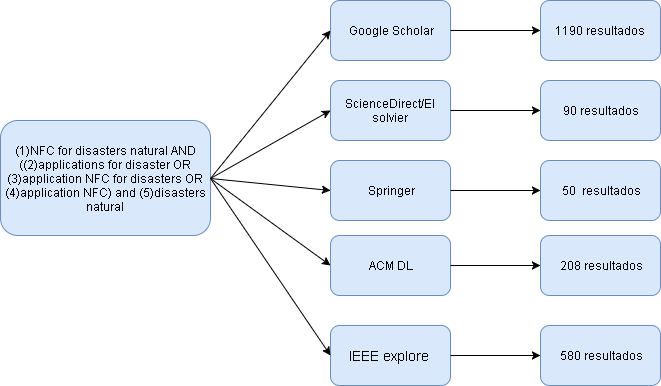
\includegraphics[width=0.9\textwidth]{imagenes/fuente.png}
			\caption{Diagrama de búsqueda de información}
			\label{Busqueda_de_informacion}
	\end{figure}

	\subsubsection{Análisis de la información}
	Para tener una mejor control de los documentos se utilizó la herramienta JabRef con la herramienta se pudo clasificar por prioridad y organizarlos  mejor para poder acceder a ellos de manera fácil si fuera necesario una revisión. \\
	Se realizó una revisión sistemática de la literatura con el fin de reducir la información sobre el tema, esta revisión consiste de los siguientes pasos:

	\begin{figure}[htb]
			\centering
			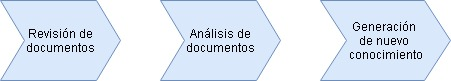
\includegraphics[width=0.7\textwidth]{imagenes/analisis.jpg}
			\caption{Diagrama de análisis de información}
			\label{Analisis_de_informacion}
	\end{figure}

	\textbf{Revisión de los documentos: }Se revisó cada uno de los documentos y de acuerdo a su contenido e interés para la investigación se clasificó. También se descartó aquellos que no sean importantes para la investigación.\\
	\textbf{Análisis de documentos: }Una vez identificados los documentos potenciales se analizó detalladamente y se clasificó de acuerdo al tipo de información brindaba. Se formaron 3 grupos significativos: aplicaciones NFC, aplicación para ayudar a resolver desastres naturales y otro sobre tecnologías relacionadas a NFC. Del resultado de análisis se extrajo lo más importante y se comparó con resultados obtenidos de otros artículos.\\
	\textbf{Generación de nuevo conocimiento: }Por último se obtuvo nuevo conocimiento sobre el problema y la información obtenido se incluyó en el marco teórico que ayudo a tener clara la investigación.\\

	\subsection{Técnicas e instrumentos de recolección de datos}
	Un instrumento de recolección de datos es, según \cite{sabino} <<cualquier recurso de que se vale el investigador para acercarse a los fenómenos y extraer de ellos información>>. Debido al tipo de diseño de investigación la técnica para la recolección de datos es la entrevista no estructurada. La ventaja de la entrevista reside en que los mismo actores brindan la información relativa a su conductas, opiniones, deseos, actitudes y expectativas, nadie mejor que la misma persona para hablarnos de lo que experimenta. Las  preguntas están orientadas al problema detectado y se ejecuta mediante la conversación y en medios naturales. el investigador elabora las preguntas antes de la entrevista en base al problema y los objetivos pero durante la entrevista se puede adaptar las preguntas a diversas situaciones.

	\subsection{Fiabilidad de la investigación}
	Toda investigación esta expuesta a errores que amenazan la validez de los datos, es por eso que se deben validar los datos capturados. Se siguieron los siguientes pasos:
	\begin{itemize}
		\item Probar el formato de las preguntas elaboradas evaluando si son claras y tienen relación con la investigación.
		\item Se hizo un simulacro para evaluar la eficiencia de los entrevistadores al momento de efectuar la entrevista.
		\item Se realizó una pequeña prueba con un grupo reducido de personas para evaluar los resultados obtenidos.
	\end{itemize}

	\subsection{Técnica de análisis de datos}
	El análisis de los datos son las operaciones que se hacen para alcanzar los objetivos definidos. \\

	\begin{figure}[htb]
			\centering
			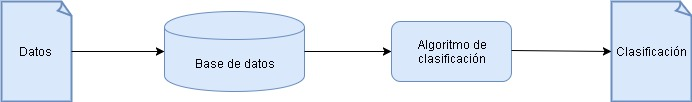
\includegraphics[width=0.9\textwidth]{imagenes/clasificacion.jpg}
			\caption{Diagrama de flujo de información para la clasificación}
			\label{Flujo_de_informacion}
	\end{figure}

	Nuestro proceso de análisis comienza ingresando los datos obtenidos de la entrevista a las bases de datos, seguido se analizan los datos y clasifica mediante el algoritmo de clasificación y por ultimo se obtiene la clasificación.


	\chapter{Marco Teórico}
	\newpage

	\section{Antecedentes de investigación}

	\subsection{Sistema de alerta para inundaciones urbanas y refugios \cite{Wister2013}}
	Es un proyecto desarrollado en la Universidad de Tabasco en México, el cual presenta un diseño inteligente para manejar la alerta de inundación urbana y refugios.\\
	En una ciudad devastada por inundaciones es común que la infraestructura de comunicación se interrumpa o sature debido al aumento de uso de las personas dificultando la comunicación con los medios de rescate. Así mismo, se podría aplicar medidas preventivas ante una inundación y tener un mejor control en los refugios debido a la gran cantidad de personas que puede alojar. Para solucionar estos problemas se plantea  tres tipos de redes, una red Ad Hoc, una red de sensores inalámbricos y una red de conexión inalámbrica que se comunican entre ellas:\\
	\textbf{Red de sensores: }Es un sistema de seguimiento del nivel del río, los sensores pueden predecir o estimar cuantos metros a subido el agua.\\
	\textbf{Red Ad Hoc: }Apoya la información de redes de emergencia y necesidades básicas de las comunicaciones. Esta red es para el rescate después de los desastres.\\
	\textbf{Red de conexión inalámbrica: }Apoya el eficiente rescate y socorro en desastres de inundaciones. Esta red recibe notificaciones de las redes anteriores para administrar refugios y demás.\\[0.25 cm]
	En la figura (\ref{modelo_de_redes}) se muestra una vista completa del modelo de red. En primer lugar, la red de  sensores (derecho) mide el nivel del río, esta información se envía a usuarios de la red Ad Hoc, entonces los ciudadanos que viven en áreas bajas que son propensos a inundaciones reciben una alerta mensaje (aviso de inundación de flash) en sus teléfonos móviles y tomarán medidas razonables cuando ocurra el desastre. Dependiendo del tipo de protocolo disponible después de un desastre, la red inalámbrica propuestas podrían comunicarse a través de una tales como Wi-Fi, ZigBee, GPRS, Bluetooth y GPS.


	\newpage
	
	\begin{figure}[htb]
			\centering
			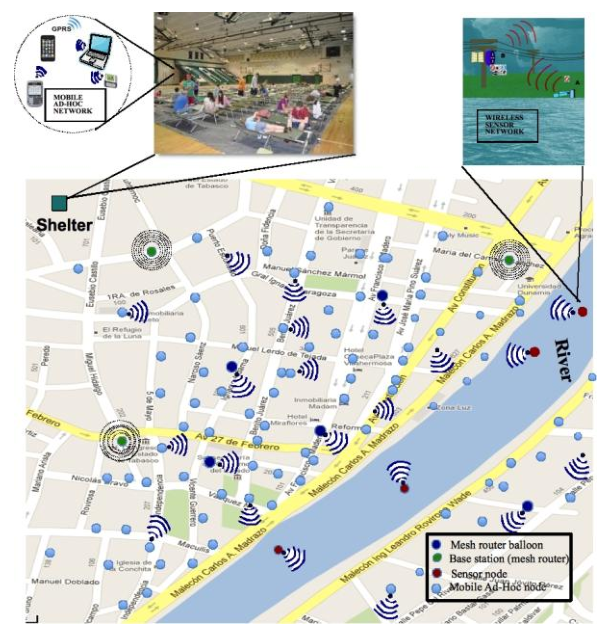
\includegraphics[width=0.9\textwidth]{imagenes/redes.PNG}
			\caption{Modelo de redes en conjunto}
			\textsl{Fuente }\cite{Wister2013}
			\label{modelo_de_redes}
	\end{figure}

	\subsection{Prototipo basado en pulseras RFID \cite{Wister2015}}
	Es un prototipo desarrollado en la Universidad de Tabasco en México para gestionar información de refugios en caso de emergencia y control de recursos entregados a los refugiados.\\

	Los refugios temporales tienen una estructura servicios de coordinación porque deben ofrecer servicios de control y actualización diaria, carnet para el control del suministro de comida, colchones, mantas y paquetes de aseo. Adicionalmente, los refugios pueden ofrecer servicios adicionales tales como atención médica, educación, recreación, puericultura, seguridad, comunicación y  transporte. La mayoría de las entradas de archivos de registro en refugios temporales se llevan a cabo en formatos impresos, para que podamos conocer el número de personas y controlar los  servicios básicos brindados durante su estancia, el control de la distribución de alimentos y entrega de artículos de tocador. Algunos problemas en el manejo de estos documentos son: posibilidad de pérdida, errores en la escritura (nombre, edad, familia, lugar de origen) y lento consultas.\\
	Se tendrá en cuenta que el gobierno instalará alojamiento temporal en edificios públicos o tiendas para apoyar a personas cuyas casas hayan sufrido daños. Hay algunas consideraciones claves:
	\begin{itemize}
		\item Proporcionar protección contra el clima.
		\item Garantizar la privacidad y la dignidad.
		\item Proporcionar seguridad.
		\item Proporcionar alimentos y camas.
	\end{itemize}
	La ayuda brindada por el  refugio debe de ser apropiada al contexto, se debe tomar en cuenta el tipo de daño causado por el desastre, estos refugios proporcionan urgencia a corto plazo a los damnificados. Este proyecto propone un prototipo para la identificación de individuos mediante el uso de la tecnología RFID, primero se escriben en una etiqueta de pulsera RFID la identificación de los damnificados, entonces la escritura/lectura se hacen según los servicios recibidos en el refugio de emergencia y se almacenan en una base de datos que se actualizará automáticamente.\\
	Este prototipo cumple con estos requisitos:
	\begin{itemize}
		\item Registro de personas en el refugio.
		\item Registro de servicios de alimentos y recursos entregados.
		\item Control de llega y salida del refugio.
		\item Control de artículos de tocador entregados.
	\end{itemize}


	\subsection{FastTriaje \cite{HernandezGoya2014}}
	Es un trabajo presentado por la Universidad de La Laguna de España, presenta un sistema de clasificación de víctimas en situaciones de emergencia que consta de una plataforma web y una aplicación móvil e integra comunicación wifi y NFC.\\
	El sistema presentado en este trabajo se denomina FastTriaje
	y se basa en el método START (Simple Triage and Rapid
	Treatment) que clasifica según su estado de gravedad y asigna colores:

	\begin{itemize}
		\item \textbf{Negro: }Víctima mortal o irrecuperable.
		\item \textbf{Rojo: }Víctimas que requieren atención médica inmediata.
		\item \textbf{Amarillo: }Víctimas que requieren cuidados urgentes, pero su estado permite un retraso en la atención de entre media a una hora.
		\item \textbf{Verde: }Víctimas que no están seriamente heridas, su tratamiento puede retrasarme a más de una hora.
	\end{itemize}

	Este método persigue dos metas esenciales en
	situaciones de emergencia y/o desastres naturales: salvar el
	mayor número de vidas posible y, simultáneamente, optimizar
	el uso de los recursos materiales y humanos disponibles, ya que en una situación de emergencia la ayuda es a menudo para un gran número de personas. Con FastTriaje el proceso completo de diagnóstico de
	la gravedad del paciente es guiado por la aplicación. El sistema
	indicará al diagnosticador el resultado final de la evaluación,
	así como la decisión que debe tomarse.\\
	Uno de los elementos del sistema es una aplicación
	móvil desarrollada para dispositivos Android. Dicha aplicación
	será la herramienta principal del personal a cargo de la evaluación del paciente, tanto a la hora de realizar su clasificación, que se realiza dependiendo de la gravedad de la persona, como también para gestionar la información generada en cada
	triaje. Una de las posibilidades incluida en la aplicación es almacenar la información asociada al triaje en una etiqueta
	NFC que se asociará al paciente. Dicha información puede
	ser consultada posteriormente en cualquier momento a través
	de la misma aplicación.
	El segundo pilar del sistema desarrollado es una plataforma
	web cuya función principal es centralizar la recogida de
	información generada por el uso de la aplicación móvil y
	facilitar la gestión de la misma, incluyendo la gestión de
	usuarios y sus privilegios.
	La aplicación móvil y la plataforma web interactúan a través
	de un servicio web REST, siendo el formato seleccionado para
	la comunicación de mensajes JSON.
	Se han incluido métodos de autenticación robusta basados
	en criptografía ligera para la comunicación de la aplicación
	con la etiqueta NFC y también con la plataforma web.

	\subsection{Control de acceso de personas\cite{Cherrez2010}}
	Prototipo presentado por la Universidad Nacional de Quito. Este prototipo tiene como finalidad realizar un control automático en el acceso de personas mediante teléfonos celulares compatibles con tecnología NFC, esto sin la necesidad de manejo y control de alguna persona sino un sistema que opere por sí sólo y permita el ingreso solamente a personas autorizadas a una determinada zona.\\
	\begin{figure}[htb]
			\centering
			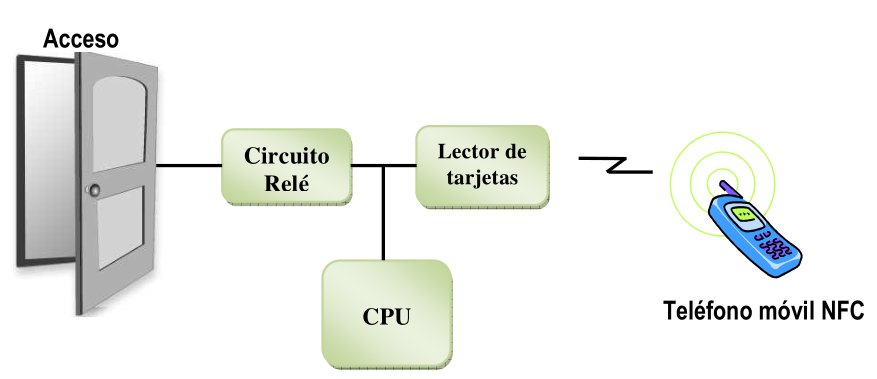
\includegraphics[scale = 0.5]{imagenes/control_acceso.PNG}
			\caption{Diagrama general del prototipo}
			\textsl{Fuente }\cite{Cherrez2010}
			\label{Diagrama_del_prototipo}
	\end{figure} \\
	Como se observa en la figura (\ref{Diagrama_del_prototipo}), se presenta el funcionamiento del sistema. Para la comunicación se utilizó el API J2ME de Java que permite el desarrollo de aplicaciones para teléfonos móviles. Esta API se basa en la especificación JSR-257 de Java que contiene los paquetes necesarios para realizar las acciones de conexión, escucha, lectura, escritura. La validación se hace en un computador a través de el lector de tarjetas, una vez que se verifica a el usuario se genera un impulso de voltaje que llega al relé que se activa con 5 VDC para activar el acceso y permitir el ingreso.

	\subsection{Control de asistencia en universidades \cite{Chulde2014} }
	Proyecto presentado por la Universidad Tecnológica Israel en Quito. El proyecto cubre el estudio, diseño e implementación de un sistema que utiliza tecnología NFC para el control de asistencia de los alumnos de la universidad. El sistema fue implementado con herramientas de software de licencia libre y un dispositivo lector/escritura NFC.El problema principal es el control de la asistencia que se realiza de forma manual y de esta manera no se tiene información de la asistencia de los alumnos en tiempo real, el alumno tiene que esperar información del docente para saber sus asistencias. En la solución se utilizó etiquetas NFC FeliCa de lectura y escritura, el lector fue le NFC Reader 122u el cual se conecta mediante puerto USB a la computadora para registrar la asistencia.\\

	El proyecto es el de la Universidad Politécnica de Madrid\cite{CondeGomez2017} , presenta un prototipo que controle la asistencia mediante tarjetas NFC utilizando el carnet universitario de los alumnos que cuenta con un chip NFC. Se utilizó C como lenguaje de programación y la biblioteca libnfc la cual tiene el estándar ISO/IEC 14443:210, también se utilizó un NFC USB reader para lectura de las tarjetas y por ultimo, se utilizó openSSl para las operaciones criptográficas.

	\subsection{Logística y pago con NFC \cite{Benyo2007,Benyo2009}}
	StoLPaN Store Logistics and Payment with NFC (Logística y pago con NFC) es un consorcio paneuropeo de empresas, universidades y usuarios. La combinación de teléfonos  con tecnología NFC hace posible una variedad de oportunidades de negocio como son: pago, ticketing, control de acceso, distribución de contenido, publicidad inteligente, transferencia de dinero. StoLPaN tiene como objetivo definir una metodología uniforme para gestionar múltiples servicios independientemente del tipo de teléfono y la infraestructura de soporte utilizada. El uso de una metodología común ayuda a reducir el costo de lanzar nuevas aplicaciones NFC eliminando la necesidad de desarrollar, certificar y administrar múltiples versiones, y permite a los usuarios crear una experiencia consistente y conveniente en todos los servicios NFC en su móvil.\\
	\textbf{Técnica de StoLPaN: }Para aplicar la metodología deben considerar los siguientes procesos:
		\begin{itemize}
			\item Evaluar como NFC afecta la cadena de valor existente para la emisión de tarjetas de pago, tránsito de boletas y otros.
			\item Identificar los requisitos de negocio.
			\item Verificación de las dependencias comerciales y a partir de esto será posible definir las reglas de negocio y los requisitos técnicos que sentarán las bases para un entorno NFC.
		\end{itemize}			
	En cuanto a la implementación, el host debe de ser capaz de soportar múltiples servicios NFC, acceso a los recursos del teléfono y facilitar la carga, uso, mantenimiento y eliminación a través de NFC. Para realizarlo se implementa:
	\begin{itemize}
		\item API común entre la aplicación y sistema operativo. Esto con el fin de proporcionar una aplicación única para cada dispositivo.
		\item API común entre el proveedor de servicios y la plataforma simplificando la validación.
		\item Interfaz de usuario común para simplificar la curva de aprendizaje.
	\end{itemize}
	En la figura (\ref{concepto_de_host}) se muestra un modelo del concepto de relación entra la  interfaz de usuario, las diferentes aplicaciones NFC y el uso de los servicios en el host.
	\begin{figure}[htb]
			\centering
			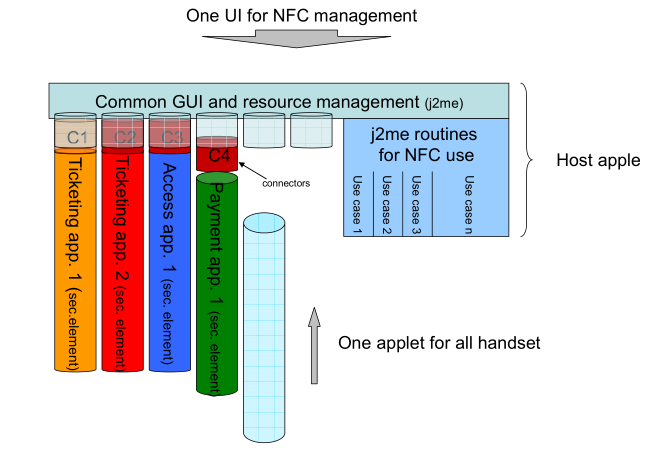
\includegraphics[scale = 0.6]{imagenes/host.PNG}
			\caption{Concepto de aplicaciones en host}
			\textsl{Fuente }\cite{Benyo2007,Benyo2009}
			\label{concepto_de_host}
	\end{figure}
	\newpage
	El producto final será un conjunto de servicios en un entorno de venta inteligente completo, el cual se basa en el etiquetado de productos con etiquetas NFC y la implementación de aplicaciones NFC. El objetivo principal es el proceso de pago como se puede ver en la imagen.
	\begin{figure}[htb]
			\centering
			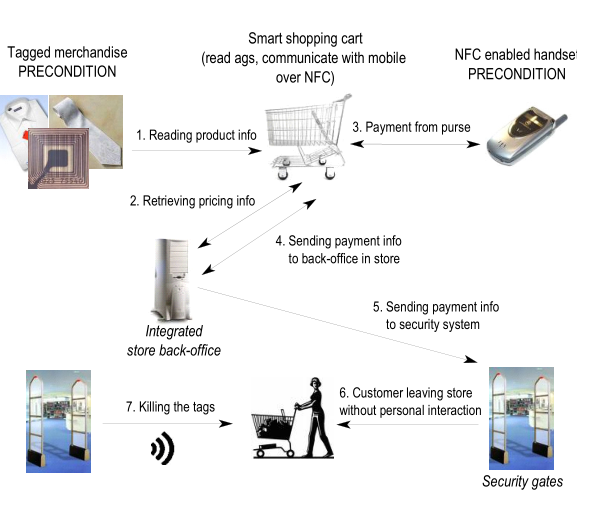
\includegraphics[scale = 0.6]{imagenes/sistema_NFC.PNG}
			\caption{Proceso de pago basado en NFC}
			\textsl{Fuente }\cite{Benyo2007,Benyo2009}
			\label{Sistema_NFC}
	\end{figure}
	\newpage

	\section{Marco conceptual de la Investigación}

	\subsection{Fenómeno Natural}
	Es toda manifestación de la naturaleza \cite{romero1993} y se refiere a cualquier comportamiento de la naturaleza. Lo hay de cierta regularidad, como son las lluvias en los meses de verano, y los de aparición extraordinaria como son los terremotos, un tsunami, una lluvia torrencial. Los fenómenos naturales de aparición extraordinaria pueden ser previsibles o imprevisibles, dependiendo del grado de conocimiento que se tenga del fenómeno. La ocurrencia de un fenómeno natural necesariamente no provoca un desastre natural, puesto que la tierra esta en proceso de formación y que su funcionamiento da lugar a cambios en su faz, los fenómenos deben ser considerados siempre como elementos activos de la geomorfología terrestre.\\
	Un desastre natural es la correlación de fenómenos naturales peligrosos (terremoto, un huracán, un maremoto, etc) y determinadas condiciones socio-económicas y físicas vulnerables (como situación económica precaria de la vivienda). En términos puntuales un fenómeno natural se vuelve un desastre si ocurre en situaciones vulnerables.\\
	\textbf{Situación vulnerable: }Ser vulnerable aun fenómeno natural es ser susceptible de sufrir daño y tener dificultad de recuperarse. No toda situación en que se halla el ser humano es vulnerable, hay situaciones en que una población sí está realmente expuesta a sufrir daños si ocurriera un evento natural, en cambio, otras poblaciones están rodeadas en condiciones seguras por lo que son consideradas 	protegidas. La vulnerabilidad se da por los siguientes puntos:
	\begin{itemize}
		\item Cuando la gente ha ido poblando terrenos que no son buenos para vivienda, por el tipo de suelo, por su ubicación expuesta a huaicos, avalanchas, deslizamientos, inundaciones, etc.
		\item Cuando no existen condiciones económicos que permitan satisfacer las necesidades humanas (no cuente con un hábitat adecuado). Esta falta de condiciones socio-económicas se debe al desempleo o subempleo teniendo como consecuencia ingresos insuficientes, escasez de bienes, entre otras.
		\item Cuando se ha construido casas precarias, sin buena base o cimientos, de material inapropiado para la zona.
	\end{itemize}
	Todos estos elementos son causantes de la vulnerabilidad física que presentan algunos pueblos, si los hombres no crean un hábitat seguro para vivir es por dos razones: la necesidad extrema o la ignorancia.\\
	Cuando ocurre un fenómeno en una situación vulnerable es cuando se da origen a un desastre natural.

	\subsection{Desastre Natural}

	Un desastre natural es una situación de daño que afecta la vida de un ecosistema\cite{vargas2002}. El daño de un desastres esta relacionado con la capacidad de protección y recuperación de su población.
	\subsubsection{Clasificación de los desastres}
	Según el origen de los desastres naturales se pueden clasificar en 2 categorías:
	\begin{itemize}
		\item \textbf{Desastres naturales: }Ocurren debido a un fenómeno natural realizando su ciclo natural, o por la intervención del hombre, se dividen en tres tipo:
		\begin{itemize}
			\item Meteorológicos: Relativos al clima y atmósfera.
			\item Topográficos y geotécnicos: Relativos a la superficie de la tierra.
			\item Tectónicos o geológicos: Relativos a lo interno de la tierra.
		\end{itemize}
		\item \textbf{Desastres antrópicos y sociales: }Es de origen humano y social y tiene la siguiente clasificación:
		\begin{itemize}
			\item Exclusión Humana: Cuando no se tiene las condiciones básicas para la existencia humana.
			\item Guerra y delincuencia: Causado por el abusivo destructivo de los humanos.
			\item Mal manejo de recursos y desecho: Explotación excesiva de los recursos para su existencia.
			\item Accidentes: Debido a un descuido en el manejo de la tecnología.
		\end{itemize}
	\end{itemize}

	La imagen (\ref{Desastres}) muestra el tipo de desastre según su clasificación.

	\newpage

	\begin{figure}[htb]
			\centering
			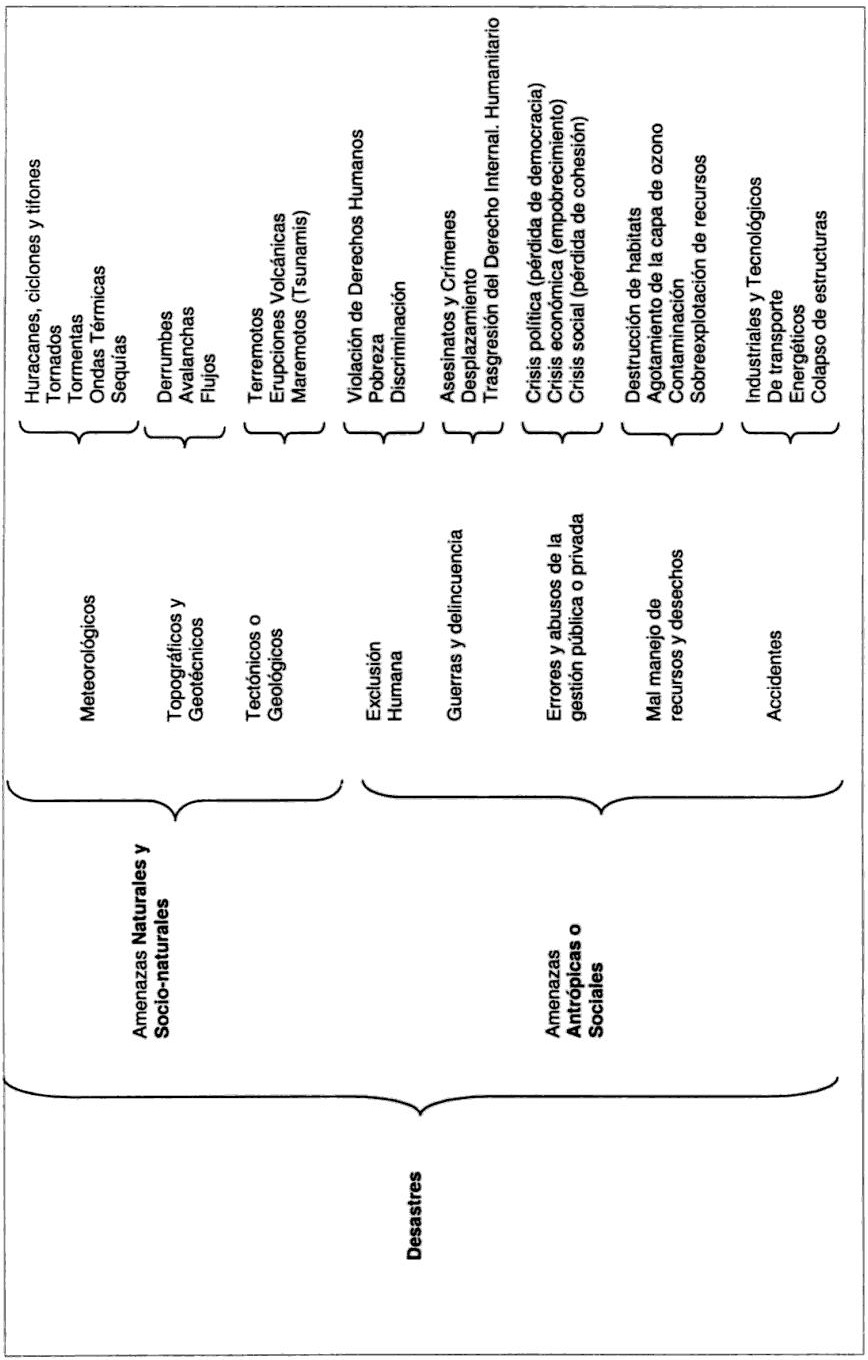
\includegraphics[width=0.6\textwidth]{imagenes/desastres.jpg}
			\caption{Tipología de desastres según su origen}
			\textsl{Fuente} \cite{vargas2002}
			\label{Desastres}
	\end{figure}

	\subsection{Recuperación de un Desastre}
	Existe modelos para representar el proceso de como una sociedad se recupera de un desastre \cite{Al-Akkad}, siendo el modelo más conocido el de Powell que propone dividir en 8 etapas un desastre.
	
	\begin{table}[htbp]
			\begin{tabular}{|l|p{9cm}|}\hline
				\textbf{ETAPA} &  \textbf{ACTIVIDAD} \\ \hline
				\textbf{Pre-desastres} & Denota el periodo de tiempo antes de que surja el desastre.\\ \hline 

				\textbf{Alerta}  & Se informa a la población potencialmente afectada, puede no haber advertencia.\\ \hline

				\textbf{Amenaza} & Cuando la población es informada del riesgo y toma medidas preventivas.\\ \hline 

				\textbf{Impacto} &Denota el clímax de un desastre. \\ \hline

				\textbf{Inventario} &La población se adapta a lo que sucedió y acuerdan colectivamente un curso de acción. \\ \hline

				\textbf{Rescate} &Las personas se ayudan a sí mismas a las que estén cerca. \\ \hline

				\textbf{Remedio} &Ayuda de profesionales, ingresan a la zona del desastre. \\ \hline

				\textbf{Recuperación} &Restauración de las propiedades. \\ \hline

			\end{tabular}
				\caption{Modelo de Powell}
		\end{table}

	\subsection{Tecnología Inalámbricas}
	Las tecnologías inalámbricas están incluidas en nuestras vidas cotidianas tanto que es difícil imaginar, por ejemplo, un celular que no cuente con Bluetooth para la transferencia de datos. Esta importancia se debe a lo fácil que han logrado la comunicación entre dispositivos olvidándonos de los cables y garantizando la seguridad de los datos.

	\subsubsection{Bluetooth}
	Es una tecnología inalámbrica de corto alcance y formar parte de WPAN (Wireless Personal Area Network) con estándar IEEE 802.15.1 permitiendo una interoperabilidad y fácil conexión entre dispositivos. Opera en la frecuencia de radio libre ISM de 2.4GHz a una velocidad de 25mbps (versión 3 de bluetooth) siendo capaz de atravesar obstáculos hasta unos 10 metros de distancia teniendo un bajo consumo de energía, originalmente surgió como una alternativa a tecnologías de cableado como RS-232  y de contar con una misma estructura de comunicación entre varios dispositivos \cite{Chavarria2011,VicenteGarcia2011}.\\
	Fue creado en 1994 por Ericsson con el fin de facilitar el intercambio de información de dispositivos como computadoras, móviles, PDAs, mas adelante, en 1999 se creo SIG de Bluetooth (Special Interest Gruop) con la unión de Ericsson, Nokia, Toshiba e IBM \cite{Bluetooth}.\\
	\textbf{Especificaciones de Bluetooth}
	\begin{itemize}
		\item Una red de bluetooth se llama Piconet con un número máximo de ocho personas siendo un dispositivo quien controla el inicio y la comunicación.
		\item Puede haber un número mayor a 8 usuarios pero pasan a un estado de inactivos y se les llama Parked.
		\item El conjunto de Piconets se le llama Scattnet.
		\item Utiliza duplexación por división de tiempo volviendo así un mismo canal para emitir y recibir mensajes controlado por tiempos.
		\item Utiliza la técnica FHSS (Frequency hoppingspread spectrum) para dividir la frecuencia 2,4 GHz en 79 canales con un ancho de banda de 1 MHz cada uno (este proceso son llamados saltos de línea) así evita interferencia con señales de radio y  evita el ruido a través de los saltos de línea.
		\item Utiliza modulación FSK Gaussiana para aumentar el ancho de banda. y ganar velocidad de transmisión.
		\item Cuenta con dos tipos de transferencia: Enlace Sincrónico orientado a Conexión y Enlace Asincrónico no Orientado a la Conexión.
	\end{itemize}

	Existen tres tipos de conectores:

	\begin{table}[htbp]
			\begin{tabular}{|l|l|l|l|}\hline

				\textbf{Transmisor} & \textbf{Potencia (mW)} & \textbf{Potencia (Dbm)} & \textbf{Alcance} \\ \hline
				Clase 1 & 100 mW & 20 dBm & 100 m \\ \hline
				Clase 2 & 2.5 mW & 4 dBm & 10 m \\ \hline
				Clase 3 & 1 mW & 0 dBm & 10 cm \\ \hline

			\end{tabular}
				\caption{Clase transmisores Bluetooth}
		\end{table}

		\textbf{Versiones de Bluetooth}\\
		\textbf{Bluetooth 1.0 y 1.0B}\\
		Primera versión lanzada que tuvo varios problemas, uno de los principales fue que los fabricantes de dispositivos tuvieron problemas para hacerlo interoperable. Esta versión tenia un hardware obligatorio para la dirección del dispositivo lo que retrasaba el funcionamiento de los dispositivos bluetooth.\\

		\textbf{Bluetooth 1.2}\\
		Esta versión fue ratificada con el estándar IEEE 802.15.1-2005. Tiene compatibilidad con la versión anterior pero con una mejora en la conexión y búsqueda de dispositivos. Sus principales características son:
		\begin{itemize}
			\item Velocidad de transmisión de 721 KBPS.
			\item Control de flujo y modos de retransmisión para L2CP (Logical Link Control and Adaptation Protocol) que incluye segmentación y re-ensamblado de paquetes.
			\item Utiliza AHF (Adaptive frequency Hopping Spread Spectrum) para evitar problemas con el ruido y así poder existir junto a otras tecnologías como WiFi.
			\item Ofrece una mejora en la calidad de enlaces de audio permitiendo la retransmisión de paquetes corruptos.
			\item Cuenta con una interfaz de controlador Host para comunicarse con el sistema operativo de una computadora.
		\end{itemize}

		\textbf{Bluetooth 2.0}\\
		Tiene compatibilidad con la versión anterior e implementa un índice de datos mejorados (EDR, Enhanced Data Rate) que permite una mayor velocidad de trasmisión, de hasta 3 mbps, y utiliza modulación por desplazamiento en frecuencia Gaussiana para obtener ancho de banda adicional para aumentar la velocidad. Tiene un ciclo de servicio menor por eso consume menos energía.

		\textbf{Bluetooth 2.1}\\
		Compatible con la versión anterior, tiene las siguientes características:\\
		\begin{itemize}
			\item Cooperación con tecnología NFC, cuando un campo NFC está disponible se crea una conexión seguro bluetooth.
			\item Permite emparejamiento simple y seguro (SSP, secure simplo pairing) obteniendo una mejora en el emparejamiento.
			\item Respuesta de investigación extendida (EIR, Extended Inquery response), se agregó mas información al momento de realizar la investigación, en donde se envían y reciben solicitudes permitiendo un mejor filtrado.
			\item Encriptación pause/resumen (ERP, encryption Pause/resume), al momento de generar una clave de encriptación no se detiene el proceso, se asegura que se transfieran los datos mientras se cambia la clave de encriptación.
			\item Consumo disminuido hasta 5 veces.
		\end{itemize}
		\textbf{ Bluetooth 3}\\
		Aumento la velocidad de transmisión hasta 24 Mbps y coopera con Wifi para que smartphones obtenen mayor velocidad de conexión.\\

		\textbf{Seguridad en Bluetooth \cite{Cherrez2010}}\\
		La seguridad en bluetooth se controla mediante claves de encriptación, antes de la versión 2.1 no existía métodos de seguridad. Existen tres modos.	
		\begin{itemize}	
			\item \textbf{Sin seguridad: }Los mecanismo de seguridad están deshabilitados y permite que cual dispositivo se conecte.
			\item \textbf{Seguridad a nivel de servicio: }Se activa luego de definir el canal, es el más apropiado para la ejecución de aplicaciones con sus requerimientos de seguridad.
			\item \textbf{Seguridad a nivel de enlace: }Se activa antes de definir el canal y es el mas seguro ya que los datos van seguros desde antes de la conexión.
		\end{itemize}

		Existen también un método seguro entre los dispositivos, consta de un numero PIN de 16 digitos que debe ser verificado en el dispositivo destino.

	\subsubsection{RFID}
	RFID (Radio Frequency Identification) o identificación por radio frecuencia, es una tecnología inalámbrica que se utiliza para la identificación de personas u objetos en diferentes bandas (de 125 KHz a 2,45 GHz) con un rango hasta 100 metros de distancia y una velocidad de 10 Mbps \cite{Cherrez2010,Chavarria2011,pdf2}. No se conoce cuando se desarrolló RFID, pero hay antecedentes que indican que se empezó en al segunda guerra mundial en donde se utilizaba para reconocer aviones enemigos o amigos.\\[0.25cm]
	\textbf{Especificaciones RFID}\\[0.25cm]
	RFID forma parte de las Auto ID ( Identificación Automática) que se utiliza para identificación, localización rastreo y monitorio de personas u objetos.
		\begin{itemize}
	\item Trabaja con diferentes radiofrecuencias 9-135KHz, 13,56 MHz, 433-860-960 MHz y 2,45 MHz.
	\item Existe 3 tipos de etiquetas:
		\begin{itemize}
			\item Activas: Emiten información y necesitan una fuente de alimentación pudiendo transmitir señales más potentes, esta fuente de alimentación puede llegar a durar varios años.
			\item Pasivas: Solo se activan ante la presencia de un lector que genera una pequeña corriente eléctrica suficiente para generar una respuesta.
			\item Semi-pasivas: Utilizan una batería interna para alimentar el microchip y responden más rápido que unas pasivas.
		\end{itemize}
-	Tiene diferente distancia de lectura y escritura para las etiquetas pudiendo llegar a los 100 metros de distancia.
-	La memoria interna generalmente es de y 32 kbytes.
	\end{itemize}

	\textbf{Banda de Frecuencia}\\[0.25cm]
	La banda depende del tipo de aplicación, se agrupa en 4 rangos:
	\newpage

	\begin{table}[htbp]
		\centering
		\begin{tabular}{|p{2cm}|p{5cm}|p{6cm}|}\hline
			\textbf{Frecuencia} & \textbf{Características} & \textbf{Aplicación}\\ \hline
			9 - 135 KHz & Banda que se puede utlizar en   & Control de acceso\\
			& todo el mundo debido a su & Identificación de animales\\
			 & alcance que es menos de 1 metro. & Control antirobo de choches.\\ \hline
			 13,56 MHz & Tiene compatibilidad con  & Control de acceso\\
			  & NFC y no tiene restricciones & Bibliotecas y control de documentación\\
			   & & Pago en medio de transporte \\
			   & & Control de equipaje en aviones\\ \hline
			   433-860-960 & Esta frecuencia tiene & Cadenas de suministro. \\
			    MHz & restricciones y no tiene una  & Trazabilidad de objetos de valor\\
			    & regulación mundial & Control anti-falsificación\\
			    & & Automatización de las tareas de inventario \\
			    & & PAgo de peajes en autopistas\\ \hline
			    2,45-5 GHz & No tiene restricciones y son & Pago de peajes\\
			    & utilizadas por etiquetas activas ya que permite la lectura a una gran distancia y altas velocidad de transmisión & Rastreo de vehículos\\ \hline
		\end{tabular}
		\caption{ Características según frecuencia}
		\textsl{Fuente \cite{Cherrez2010,garde2016}}
	\end{table}

	\textbf{Arquitectura RFID}\\[0.25cm]
	Una arquitectura RFID tiene los siguientes elementos:
	\begin{itemize}
		\item \textbf{Lector RFID: }Está compuesto por una antena, una unidad de control, un transceptor y un decodificador \cite{Cherrez2010}. El lector enviá periódicamente señales para rastrear etiquetas para interactuar, cuando se realiza el enlace con la etiqueta el lector extrae la información de ella y lo pasa al Middleware RFID. El lector también da energía a las etiquetas pasivas y semi-pasivas.
		\item \textbf{Middleware RFID: } Subsistema que da servicios para el procesamiento y almacenamiento de datos.
		\item \textbf{Etiqueta RFID: }Conocido también como tag, esta formado por una antena, un transductor de radio, un microchip donde se guarda la información y, dependiendo del tipo de etiqueta, una batería \cite{Cherrez2010}. Las etiquetas transportan la identificación de objeto y la información, existen diferentes modos de trabajo:
		\begin{itemize}
			\item \textbf{Solo Lectura: }La información se almacena en la fabricación y no puedo ser modificada.
			\item \textbf{Lectura Escritura: }Es ta etiqueta mas usada pero tiene un mayor precio que la anterior, permite la lectura y modificación de la información.
			\item \textbf{Anti-colisión: }Tipo de etiquetas que permite que un lector puede leer varias de su tipo sin que ocurra algún error.
		\end{itemize}
		\item \textbf{Antena: }Es un elemento importante en la transmisión ya que de ella depende el alcance, la cobertura y precisión de los datos enviados. Depende de su ubicación y el diseño que tenga.
	\end{itemize}

	\textbf{Seguridad}\\[0.25cm]
	Los sistemas basado en RFID tiene una vulnerabilidad al momento de enviar los datos ya que no cuentan con una encriptación, lo que implica que se pueda interferir la señal y se puede acceder a la información dependiendo de la distancia. En un ambiente de comercio se podría cambiar las etiquetas, el precio de productos, y aprovechar de esta desventaja, por ejemplo, cambiar etiquetas de un producto de calidad y de costo elevado por uno de menor costo. También se podría modificar la integridad de los datos de la etiqueta ya que no cuenta con una encriptación. Las formas de ataque a RFID podrían ser varias pero la tecnología ha ido creciendo y generando millones de ganancias y se implementarán nuevas medidas de seguridad.

	\subsubsection{Zigbee}

	Es una tecnología que pertenece a las redes inalámbrica de área personal (WPAN), tiene estándar IEEE 802.15.4 y opera en una radiofrecuencia de 868-915-2.4 GHz alcanzando una velocidad de transmisión de 25 Kbps en un alcance de 75 metros \cite{Cherrez2010,Chavarria2011,Carignano2011}. Zigbee es promovida por la Zigbee Alliance \cite{Zigbee} y esta formada por más de 100 compañias como Motorola, Mitsubishi, Philips, Samsung, Honeywell, Siemens, entre otras. \\
	El objetivo de Zigbee, además de las ventajas de una tecnología inalámbrica, es habilitar redes con capacidad de control y monitoreo de bajo consumo de energía y bajo costo, que funcione vía radio y de modo bidireccional, y esté en un estándar global que permitiendo que sea compatible con otras tecnologías. Se utiliza principalmente en el campo de la domótica.\\[0.25cm]
	\textbf{Especificaciones de Zigbee}\\[0.25cm]
	Zigbee pretende aprovechar características que otras tecnologías no brindan ,entre esas estan:
	\begin{itemize}
		\item Es más amigable con el medio ambiente ya que utiliza poca energía y aporta un ahorro a los usuarios.
		\item Ya que el consumo de Zigbee es mínimo el mantenimiento de las baterías es menos costosa ya que su vida útil es mayor.
		\item Utiliza diferentes radiofrecuencias:
		\begin{itemize}
			\item 868 MHz utilizada en Europa.
			\item 915 MHz en Norte América y Australia.
			\item 2,4 GHz utilizada en el resto del mundo.
		\end{itemize}
		\item La velocidad de transferencia varia dependiendo de la frecuencia:
		\begin{itemize}
			\item 2,4 GHz tiene una velocidad de 250 Kbps.
			\item 915 MHz tiene una velocidad de 40 Kbps.
			\item 868 MHz tiene un velocidad de 20 Mbps.
		\end{itemize}
		\item Soporta nodos desde 32 hasta 255 nodos.
		\item La seguridad ofrecida es mediante encriptación de los datos.
	\end{itemize}
	\newpage

	\textbf{Arquitectura Zigbee}\\[0.25cm]
	\textbf{Coordinador de Red: }Requiere de capacidad computacional, memoria y es el encargado de controlar el sistema y la ruta que deben seguir los dispositivos. Solo existe un coordinador por red.\\
	\textbf{Router zigbee: }Conecta a los dispositivos a la red Zigbee.\\

	\subsubsection{Tecnología NFC} 
	NFC es acrónimo de "Near Field Communication" y hace referencia a un protocolo/tecnología de comunicación de corto alcance que es inferior a 4 centímetros y cuenta con una velocidad máxima de 424 Kbps de transmisión de datos y opera sobre la radio frecuencia de 13.56 MHz siendo utilizada mundialmente de manera libre.\cite{Antonio2016,NFCrango,VicenteGarcia2011,Cherrez2010}.\\
	NFC fue desarrollada por Royal Philips y Sony Corporation en 2002 por un esfuerzo en desarrollar una tecnología que facilite la comunicación en dispositivos acoplados\cite{Al-Akkad,Anaya2015,Benyo2009}. En 2004 Nokia, Philips Semiconductors y Sony fundaron el NFC forum con 190 miembros\cite{Al-Akkad} con el objetivo de desarrollar especificaciones, estándares, arquitecturas, parámetros de inalterabilidad para el protocolo y dispositivos NFC\cite{Antonio2016}. En el 2006 Nokia desarrolló el primer dispositivo con NFC, el Nokia6131, que salió al mercado en Abril del 2006\cite{Antonio2016}, pero no fue hasta el 2009 que NFC empezó a tener un uso más amplio debido a su integración en teléfonos celulares abarcando aplicaciones en distintas áreas tales como medicina, control de accesos, publicidad, educación, identificación, control de activos, pagos móviles\cite{Anaya2015}.\\

	NFC combina tecnologías como RFID y tarjetas inteligentes para obtener una comunicación simple, segura e intuitiva entre dispositivos. Lo que hace interesante a NFC es su compatibilidad con otras tecnologías como bluetooth, RFID y Wifi \cite{VicenteGarcia2011}. NFC tiene una gran velocidad de transmisión de unos cuantos bits de información y lo realiza sin necesidad de una sincronización previa.\\
	\newpage
	\textbf{Arquitectura de NFC}\\[0.25cm]
	NFC tiene varias capas, la capa más baja es la física (hardware) donde se encuentra el CPU y los radios de comunicación. En medio se encuentran la capa de los Tags donde se definen los paquetes de transporte de datos y por último la capa de software donde se encuentra el código de aplicación. A continuación se muestra un gráfico donde se detalla estas capas.

	\begin{figure}[htb]
			\centering
			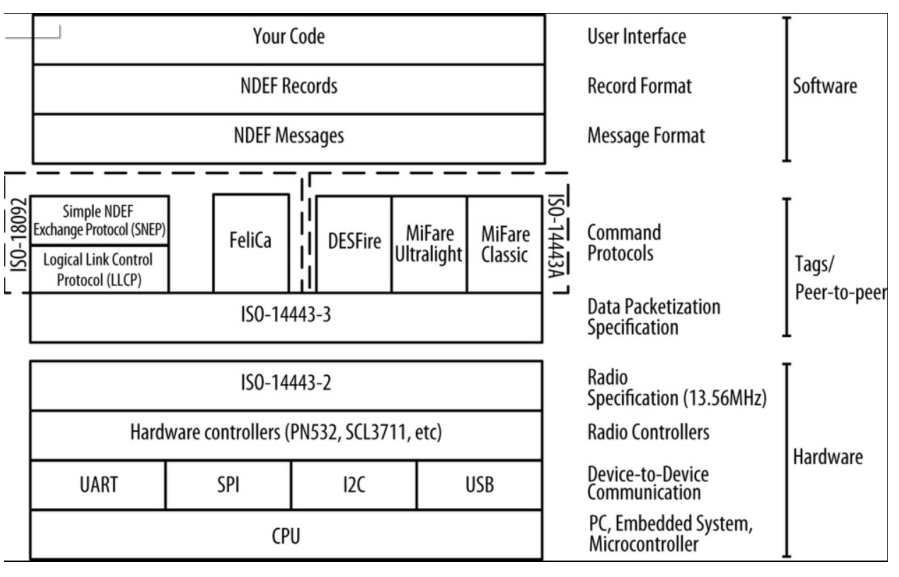
\includegraphics[width=1\textwidth]{imagenes/arquitectura_nfc.PNG}
			\caption{Arquitectura de NFC}
			\label{Arquitectura_de_NFC}
	\end{figure}

	\textbf{Formas de operar de NFC}[0.25cm]\\
	Los dispositivos NFC utilizan circuitos inductivos emparejados que intercambian información cuando están cerca entre si. Utiliza comunicación half-duplex (ambos sentidos pero no a la vez) y los dispositivos NFC verifican el campo de frecuencia para verificar si la señal recibida coincide con la enviada. Existen 3 configuraciones para utilizar NFC:
	\begin{itemize}
		\item \textbf{Emulación de tarjetas: }El dispositivo NFC se comporta como una tarjeta sin contacto y se puede utilizar las características de seguridad avanzada, como por ejemplo, hacer pagos sin contacto.
		\item \textbf{Modo Lectura: }Este es cuando un dispositivo NFC se encuentra activo y lee un tag pasivo, este modo es el más usado.
		\item \textbf{Modalidad P2P: }Dos dispositivos NFC se comunican entre sí intercambiando información.
	\end{itemize}
	\textbf{Estándares de comunicación}\\[0.25cm]
	NFC ha desarrollado formatos en común para la comunicación de dispositivos y de tarjetas:\\
	\begin{itemize}
		\item \textbf{NDEF (NFC Data Exchange Format): }Es un formato ligero de comunicación para guardar y transportar diferentes tipos de elementos. Sólo se especifica la estructura y es el mismo para dispositivos NFC o para los tags, la información de NDEF es independiente del tipo de dispositivo que se este comunicando. NDEF puede enviar desde archivos XML, datos encriptados, imágenes o cadenas de información.
		\item \textbf{RTD (Record Type Definition): }Especifica el tipo de registro que será enviado entre los dispositivos:
		\begin{itemize}
			\item \textbf{Smart poster RTD: }Etiqueta con datos como URLs, SMS o números telefónicos.

			\item \textbf{Text RTD: }Para registros que contengan solo texto.
			\item \textbf{Uniform Resource Identifier (URI) RTD: }Para registros que necesiten de internet.
		\end{itemize}
	\end{itemize}
	\textbf{Características de funcionamiento}\\[0.25cm]
	Para que NFC opere se requieren 2 dispositivos, uno que inicie la comunicación, este rol es intercambiable:
	\begin{itemize}
		\item \textbf{El iniciador (initiator): }Inicia la comunicación y controla el intercambio de información.
		\item \textbf{El objetivo (target): }Dispositivo que responde a la petición del iniciador.
	\end{itemize}
	\textbf{Modo de Funcionamiento}
	\begin{itemize}
		\item \textbf{Modo activo: }Cuando el dispositivo genera su propio campo de radio frecuencia para enviar los datos, en este modo es necesario una fuente de energía.
		\item \textbf{Modo pasivo: }El dispositivo genera la campo de frecuencia y es el dispositivo quien utiliza el campo para poder enviar los datos.
	\end{itemize}

	\textbf{Protocolos de comunicación: }\\[0.25cm]
	NfC trabaja con 2 protocolos NFCIP1 (near field comunication interface protocol-1) y NFCIP2(near field communication and protocol-2):
	\begin{itemize}
		\item \textbf{NFCIP-1: }Define la radio frecuencia con la que trabaja, en este caso 13.56 MHz, especifica la arquitectura para el envió de datos con una velocidad de 424KBPS y define el modo de operación por ejemplo la iniciación y selección de objetivo en le modo pasivo para evitar colisiones. En los sistemas NFC se pueden comunicar un máximo de 2 dispositivos  a la vez, Un dispositivo es el iniciador y tiene el rol de activo y el pasivo se llama target.
		\item \textbf{NFCIP-2: }Selecciona modos de comunicación para no interferir con otras comunicaciones en la frecuencia 13.56 MHz. Los modos para este protocolo son:
		\begin{itemize}
			\item Modo NFC
			\item Modo PCD (Proximity Coupling Devices)
			\item Modo VCD (Vicinity Coupling Devices)
		\end{itemize}
		La diferencia entre estos modos es la distancia necesario para la detección del campo de radiofrecuencia.
	\end{itemize}

	\textbf{Pasos de la comunicación}\\[0.25cm]
	\textbf{Descubrimiento: }Los dispositivos se rastrean para su reconocimiento.\\
	\textbf{Autenticación: }Los dispositivos verifican si deben establecer algún tipo de cifrado para la comunicación con el otro dispositivo.\\
	\textbf{Negociación: }Se define la velocidad de transmisión, la identificación del dispositivo, el tipo de aplicación, su tamaño, y la acción a ser solicitada.\\
	\textbf{Transferencia: }Intercambio de datos.\\
	\textbf{Confirmación: }El dispositivo receptor confirma el establecimiento de la comunicación y la transferencia de datos.\\

	\textbf{Tipo de etiquetas}\\[0.25cm]
	Una etiqueta NFC es similar a la de RFID existiendo diferentes tipos dependiendo de sus características. En el siguiente cuadros se muestra un resumen de los 4 tipos de etiquetas que existe y sus características:

	\begin{figure}[htb]
			\centering
			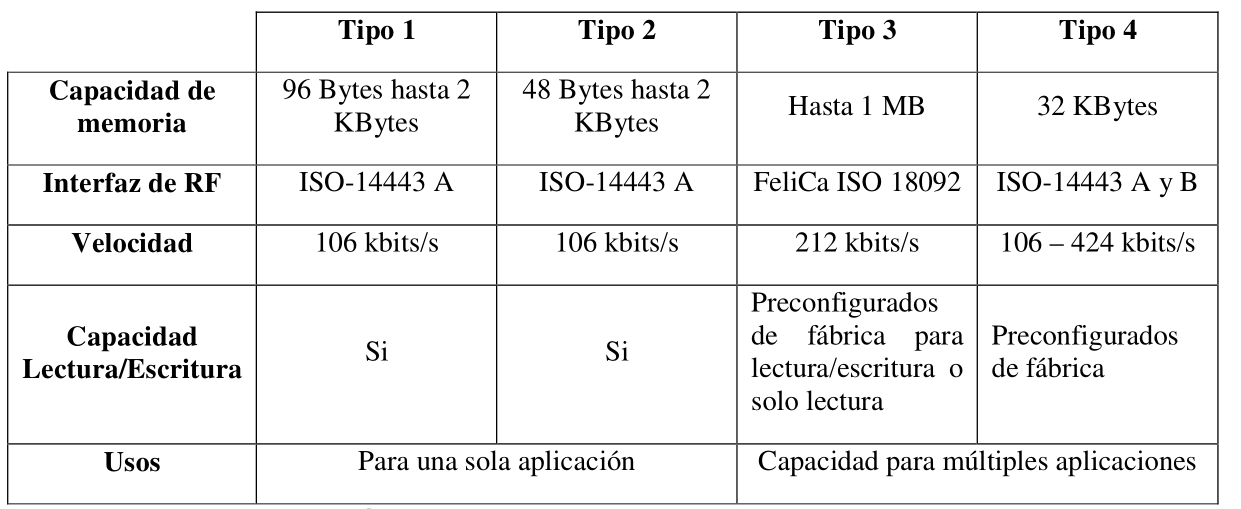
\includegraphics[width=1\textwidth]{imagenes/tags.PNG}
			\caption{Características de las etiquetas}
			\textsl{Fuente }\cite{VicenteGarcia2011,Cherrez2010}
			\label{etiquetas}
	\end{figure}
	\textbf{Seguridad en NFC}\\[0.25cm]
	Se puede considerar segura por el corto alcance para realizar la comunicación, pero es vulnerable a los equipos que estén al pendiente de escuchar la comunicación por lo que es necesaria la encriptación de los datos y proporcionar un canal seguro como SSL.\\
	Algunos ataques  son:
	\begin{itemize}
		\item \textbf{Relay-Atack: }Este ataque consiste en redirigir la información de un dispositivo a otro. Este tipo de ataque es fácil de evitar, se realiza una autenticación doble al momento de realizar la transacción aplicando firma de etiquetas.
		\item \textbf{Inicialización de servicios sin consentimiento: }Puesta en marcha del servicio son consentimiento del usuario, esto se da en un escenario en donde el bluetooth se activa y se accede a los ficheros.
		\item \textbf{Otros ataques: }Como Man in the middle, modificación y corrupción de datos, denegación de servicio o Snnifing son difícil de realizar debido al proximidad necesaria para la comunicación.
	\end{itemize}

	\textbf{Estándares internacionales}\\[0.25cm]

	NFC es compatible con cientos de millones de tarjetas sin contacto y lectores ya desplegados en todo el mundo \cite{NFC1}. La tecnología NFC está bajo estándares ISO/IEC 14443:2011 \cite{NFC2,Al-Akkad},  ISO/IEC 15693:2010 \cite{NFC3}, ISO/IEC 18092:2013 \cite{NFC2013} y cuenta con la certificación ECMA-340 \cite{ECMA,Benyo2009}.\\
	El estándar ISO/IEC 14443-3:2011 está dividido en 4 partes:

	\begin{table}[htbp]
	\begin{center}
	\begin{tabular}{|l|p{9cm}|}\hline
	\textbf{ISO/IEC 14443:2011} &  \textbf{ESPECIFICACIÓN} \\ \hline
	\textbf{14443-1} & Describe las características físicas de las tarjetas tales como el tamaño máximo de la antena y tolerancia al campo electromagnético.\\ \hline 

	\textbf{14443-2}  & Describe las características del nivel físico tales como la potencia de la emisión, la frecuencia, la tasa de bits y la modulación.\\ \hline

	\textbf{14443-3} & Describe las características del nivel de enlace tales como la forma de los paquetes de datos y el sistema anti-colisión que es usado en el descubrimiento de las tarjetas pasivas por arte del sistema activo.\\ \hline 

	\textbf{14443-4} &Describe un protocolo opcional para el nivel de transporte. \\ \hline
	\end{tabular}
	\caption{Estándar ISO/IEC 14443:2011}
	\textsl{Fuente \cite{parte1,parte2,parte3,parte4}}
	\end{center}
	\end{table}

	\newpage

	\subsubsection{Comparación de tecnologías}

	Se presenta un cuadro comparando las diferentes tecnologías.

	\begin{figure}[htb]
			\centering
			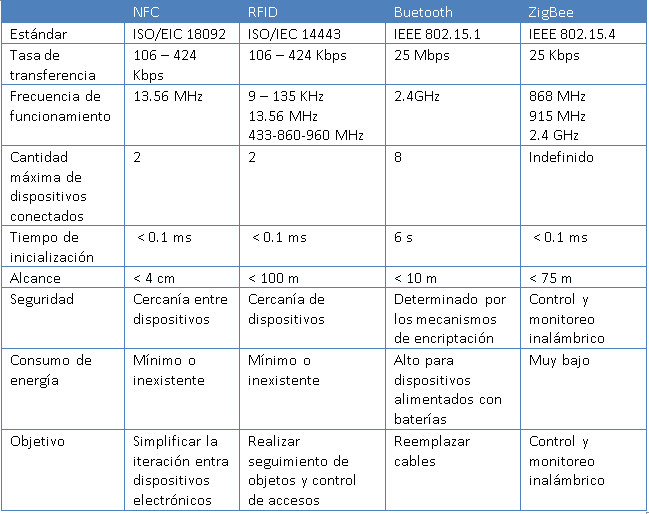
\includegraphics[width=1.1\textwidth]{imagenes/tecnologias.PNG}
			\caption{Comparación de tecnologías}
			\label{tecnologias}
	\end{figure}

	Con esta información se escogió la tecnología NFC por las siguientes razones:
	\begin{itemize}
		\item Una gran velocidad de transferencia considerando que no se escribirán datos de gran tamaño en las tarjetas NFC, los 424 Kbps que ofrece son mas que suficientes.
		\item La cantidad máxima de dispositivos conectados que ofrece NFC son 2 siendo de consideración ya que los procesos de registro y repartición serán solo entre el registrador/repartidor y damnificado.
		\item El tiempo de transferencia es menor a un segundo siendo importante en una situación de emergencia.
		\item Debido al corto alcance, 4 cm, garantiza una seguridad y permite la autenticación del damnificado. Adicionalmente se puede incluir métodos de seguridad en los tags, como encriptación de datos, y dependiendo de la tarjeta, métodos de re-autenticación.
		\item Debido al bajo consumo de energía e inexistente para los tags nfc fue escogido.
	\end{itemize}

	\subsection{Metodologías desarrolo Ágil}
	\subsubsection{Scrum}

	Es una metodología ágil basa en un marco de trabajo iterativo incremental para el desarrollo de software, productos o proyectos. Se caracteriza por utilizar los denominados Sprints o ciclos de trabajo delimitados por el tiempo.\\
	\textbf{Componentes de Scrum}\\[0.25cm]
	Scrum se divide en 3 fases, las reuniones, los roles y los elementos que la conforman:\\
	\textbf{Las Reuniones:}En un inicio las reuniones son para definir el Backlog, que es una lista de tareas que se van a realizar, y la planificación de los Sprints. Luego se realizan reuniones diariamente para conocer el progreso de trabajo y se organiza para llegar terminar las tareas restantes. Las observaciones encontradas se pueden incorporar al siguiente sprint y finalmente al finalizar un sprint se realizará una reunión con los miembros del equipo para compartir las lecciones aprendidas, dificultades en el desarrollo y recomendaciones para próximos sprints.\\ 
	\textbf{Los roles: }
	\begin{itemize}
		\item \textbf{Product Owner: }Es la persona que toma las decisiones y es la que realmente conoce el negocio del cliente y su visión del producto. Se encarga de priorizar las tareas en el backlog.
		\item \textbf{ScrumMaster: }Es el encargado de controlar el modelo y la metodología. Debe eliminar todos los procesos que impidan la interacción con el cliente y con los gestores.
		\item \textbf{Equipo de desarrollo: }Es un equipo pequeño de unas 5-9 personas y tienen autoridad para organizar y tomar decisiones para cumplir con el objetivo.
		\item \textbf{Usuarios: }Es el destinatario final del producto.
		\item \textbf{Stakeholders: }Las personas a las cuales el producto les dará algún beneficio.
	\end{itemize}
	\textbf{Elementos de Scrum: }
	\begin{itemize}
		\item \textbf{Product backlog: }Lista de necesidades del cliente.
		\item \textbf{Sprin Backlog: }Lista de tareas que se realizan en un Sprint.
		\item \textbf{Incremento: }Parte añadida o desarrollada en un Sprint, en un terminado y totalmente operativa.
	\end{itemize}
	\textbf{Características más importantes de Scrum}\\[0.25cm]
	\begin{itemize}
		\item \textbf{Flexibilidad en los entregables: }En contenido de los entregables es determinado por el entorno.
		\item \textbf{Flexibilidad en el cronograma: }Los entregables pueden ser requeridos antes o después de los planificados inicialmente.
		\item \textbf{Equipos pequeños: }Cada equipo se compone de hasta 6 miembros. El proyecto puede tener varios equipos.
		\item \textbf{Frecuentes revisiones: } EL progreso del equipo es revisado tan frecuentemente como determine la complejidad y riesgo del entorno. Se debe preparar una entrega operable en cada revisión por cada equipo.
		\item \textbf{Frecuentes revisiones: }El progreso del equipo es revisado tan frecuentemente como determine la complejidad y riesgo del entorno. Se debe preparar una entrega operable en cada revisión por cada equipo.
		\item \textbf{Colaboración: }La colaboración dentro o entre equipos es separada durante el proyecto.
		\item \textbf{Orientada a objetivos: }Cada equipo se encarga de un conjunto de objetivos, con interfaces claras y sus comportamientos.
	\end{itemize}
		\subsubsection{Extreme Programamming}
		La metodología XP también se enfoca en el desarrollo iterativo e incremental de software, se centra principalmente en el código que producen los programadores para obtener software funcional con una alta capacidad de respuesta a los cambios que se presentan durante el proyecto. Para conseguir una coordinación eficiente dentro del equipo de programadores y con los involucrados del proyecto, se promueve estos valores: simplicidad, comunicación, retro-alimentación, valentía y respeto.\\
		Estas son las características  que sobresalen en extreme programming:
		\begin{itemize}
			\item \textbf{El juego de la planificación: }Frecuentes negociaciones entre los clientes y los programadores acerca del ámbito y tiempo de los entregables.
			\item \textbf{Entregas pequeñas: }Producción rápida de versiones operativas del negocio, aunque no contengan toda la funcionalidad de los entregables.
			\item \textbf{Metáforas: }El sistema se define por historias que describen la funcionalidad del sistema, metáfora, compartidas por le cliente ayudando incluso en la nomenclatura de clases y métodos.
			\item \textbf{Diseño simple: }Las soluciones simples son las más fáciles de mantener por lo que su uso es altamente recomendado.
			\item \textbf{Pruebas: }Se diseña test al principio de cada iteración de manera que el código se determine en función del mínimo necesario para pasar las pruebas. Las pruebas son unitarias y frecuentes, realizadas por los desarrolladores.
			\item \textbf{Refactorización: }Se modifica ciertas partes del código sin cambiar su funcionalidad de manera que sea más simple.
			\item \textbf{Programación en parejas: }Aporta mejoras sustanciales a la calidad del código debido a que se puedan observar errores más rápidamente por la constante revisión a que se somete, diseños más simples, mayor dinamismo en los equipos de trabajo, mayor compresión del sistema por parte de los programadores.
			\item \textbf{Propiedad colectiva del código: }Se estimula la revisión, modificación o aportes a la funcionalidad del código, de manera que el conocimiento del sistema se comparte entre todos los integrantes del equipo.
			\item \textbf{Integración continua: }Todos los aportes en código de las parejas de programadores se integran rápidamente al sistema, de manera que puedan continuar con el desarrollo con las últimas versiones.
			\item \textbf{40 horas por semana: }De manera que no se sobrecargue ni se desmotive al equipo con exceso de trabajo, el cual puede ser un síntoma de algún problema que debe corregirse.
			\item \textbf{Disponibilidad del cliente: }El cliente debe formar parte del equipo de manera que pueda tomar decisiones sobre el código en cualquier momento y no solo en las reuniones que se planifican.
			\item \textbf{Estándares de programación: }Todos los programadores deben alinearse a estándares de programación para mantener el código simple y legible. La comunicación entre programadores se potencia mediante el código.
		\end{itemize}

	\chapter{DISEÑO E IMPLEMENTACIÓN DE LA SOLUCIÓN}
	\newpage

	\section{Definición de requerimientos}
	\textbf{Requerimientos Funcionales}

	\begin{figure}[htb]
			\centering
			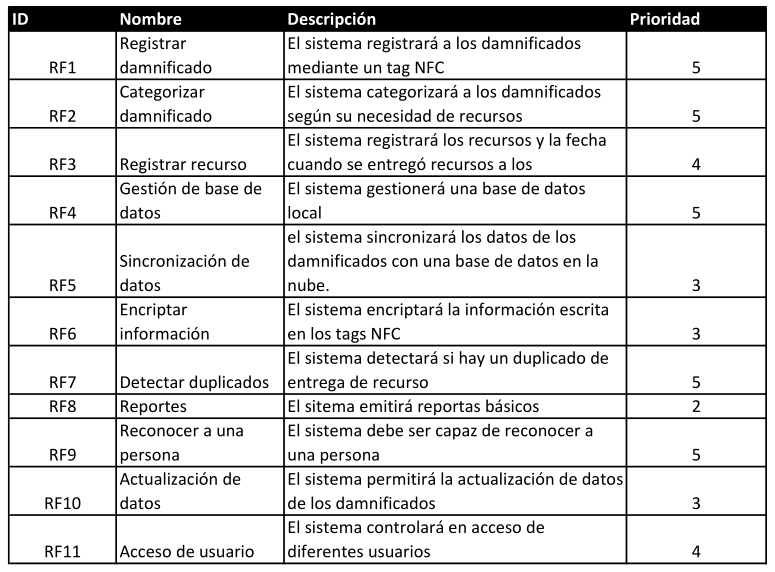
\includegraphics[width=1\textwidth]{imagenes/requisitos_funcionales.PNG}
			\caption{Requisitos funcionales}
			\label{Requisitos_Funcionales}
	\end{figure}

	\newpage

	\textbf{Requerimientos no funcionales}
	
	\begin{figure}[htb]
			\centering
			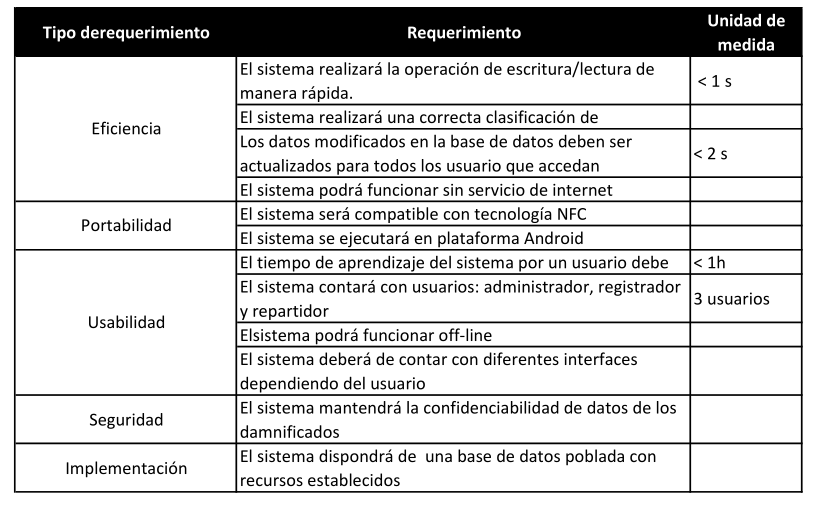
\includegraphics[width=1\textwidth]{imagenes/requerimientos_no_funcionales.PNG}
			\caption{Requisitos no funcionales}
			\label{Requisitos_no_funcionales}
	\end{figure}

	\section{Arquitectura}
	En esta sección se presenta la arquitectura, que se basa en el patrón arquitectónico Modelo-Vista-Controlador (Model View Controler) y arquitectura de microservicios.En la figura \ref{Arquitectura} se muestra las capas de la arquitectura propuesta y se describe cada una de ellas. La capa modelo del cliente se encuentra conformada de la siguiente manera:\\
	\textbf{Catálogo de elementos: }Se encarga de almacenar en el dispositivo los datos necesarios para el funcionamiento correcto de la aplicación.\\ [0.25cm]
	La capa lógica del cliente se encuentra conformada por los siguientes componentes:\\
	\textbf{Lectura: }Se encarga de gestionar la lectura de datos de las etiquetas NFC. Genera el campo de radiofrecuencia para extraer los datos.\\
	\textbf{Escritura: }Se encarga de la preparación y manipulación de datos que se requieren escribir, ya que es necesario que cumplan con requisitos previos, ente los cuales está el darles un formato adecuado y determinar el tipo de dato.\\
	\textbf{Comunicación: }Se encarga de realizar el enlace entre el dispositivo y la etiqueta.\\
	\textbf{Manejador de aplicación: }Se encarga de gestionar la ejecución de la aplicación, establece la conexión cuando el dispositivo se pone en contacto con una etiqueta NFC.\\
	\textbf{Consumidor de servicios: }Componente ubicado dentro del módulo de lógica del negocio el cual se encarga de la invocación de los servicios.\\ [0.25 cm]
	La capa de la vista cuenta con 2 componente:\\
	\textbf{Captura de datos: }Muestra las vistas necesarias para la captura de los datos.\\
	\textbf{Presentación de datos: }Muestras las vistas con la información solicitada.\\[0.25 cm]
	La capa de servicio está formada por los siguientes componentes:\\
	\textbf{Componentes : }Los componentes de la capa de servicio el cual se encarga de la interoperabilidad de aplicaciones mediante su infraestructura.\\
	\textbf{Servicio: }Atiende las peticiones de la aplicación.\\[0.25 cm]
	La capa de recursos está formada por:\\
	\textbf{Datos: }Componente encargado de almacenar y proporcionar datos.
	\begin{figure}[htbp]
			\centering
			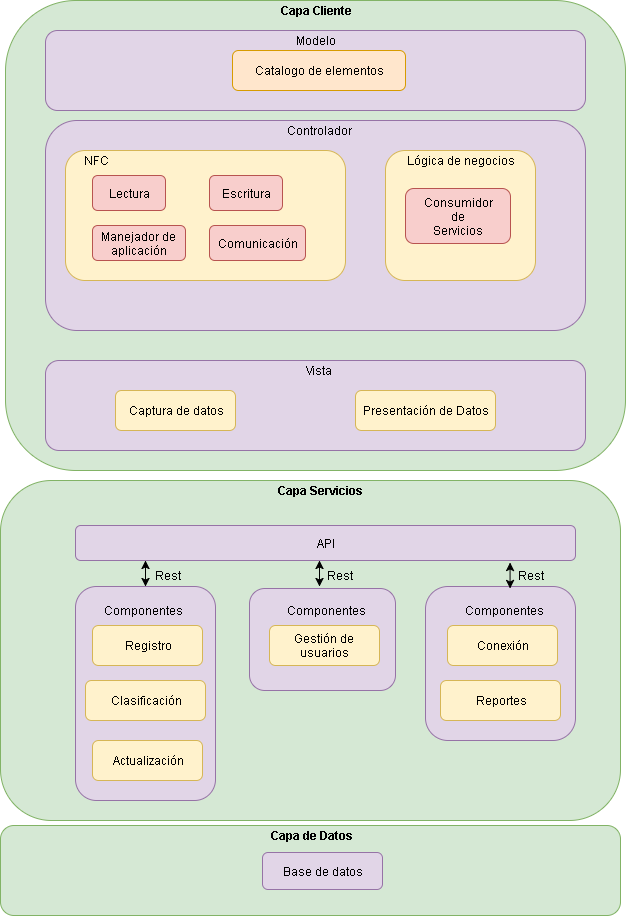
\includegraphics[width=0.9\textwidth]{imagenes/Arquitectura.png}
			\caption{Arquitectura}
			\label{Arquitectura}
	\end{figure}
	\newpage

	\section{Modelo de datos}
	A continuación se presenta el modelo de datos, en este modelo es una representación de los datos que se necesitar almacenar y en que entidades. Las entidades identificados fueron:\\[0.25cm]
	\textbf{Kit\_Recurso: }Entidad que representa a los kit de apoyo que se le brindará a los damnificados por le desastre. Se registra:
	\begin{itemize}
		\item \textbf{idKit\_Recurso: }Es un identificador único para el kit de ayuda.
		\item \textbf{Tipo: }Para identificar que tipo de recurso es, puede ser abrigo, agua, alimento.
	\end{itemize}
	\textbf{Desastre: }Entidad que representa a un desastre natural, se registra:
	\begin{itemize}
		\item \textbf{ID\_desastre: }Es un identificador único para un desastre natural.
		\item \textbf{Nombre\_Desastre: }El nombre del desastre ocurrido. 
	\end{itemize}
	\textbf{Damnificado: }Entidad que representa a los damnificados de un desastre natural. Se registra:
	\begin{itemize} 
		\item \textbf{ID\_daminificado: }Un identificador único para cada damnificado.
		\item \textbf{Foto: }Una foto del damnificado para poder reconocerlo al momento de realizar la repartición de recursos.
		\item \textbf{Nombres: }Nombres del damnificado.
		\item \textbf{Apellidos: }Apellidos de los damnificados.
		\item \textbf{Genero: }Género o sexo del damnificado registrado.
		\item \textbf{Edad: }Edad del damnificado registrado.
		\item \textbf{Celular: }Celular del damnificado, puede ser nulo en caso no tenga el damnificado.
		\item \textbf{Departamento: }Departamento de donde es el damnificado.
		\item \textbf{Distrito: }Distrito al que pertenece el damnificado.
		\item \textbf{Dirección: }Dirección del damnificado.
		\item \textbf{Estado: }Estado en el que esta el damnificado, puede ser sano, enfermo, embarazada.
	\end{itemize}
	\textbf{Tarjeta: }Entidad que representa la tarjeta con el chip NFC que se le brindará a los damnificados, se registra:
	\begin{itemize}
		\item \textbf{id\_tarjeta: }Un identificador único para cada tarjeta.
		\item \textbf{Fecha\_registro: }Fecha en la que se hizo el registro del damnificado y se le entregó la tarjeta.
		\item \textbf{Fecha\_entrega: }Fecha cuando se entregó los recursos al damnificado.
		\item \textbf{Lugar\_entrega: }Lugar en donde se realizó la entrega.
	\end{itemize}
	\textbf{Registro\_Sanidad: }Representa a una historia clínica del damnificado, se registra sus enfermedades y una breve descripción.\\
	\textbf{Enfermedad: }Enfermedad que pueda tener el damnificado, se registra el nombre y una descripción.\\
	\textbf{Usuario: }Usuario que utilizará el aplicativo, ya sea para registrar, para repartir o administrar. Se registrar sus datos.
	\begin{figure}[htbp]
			\centering
			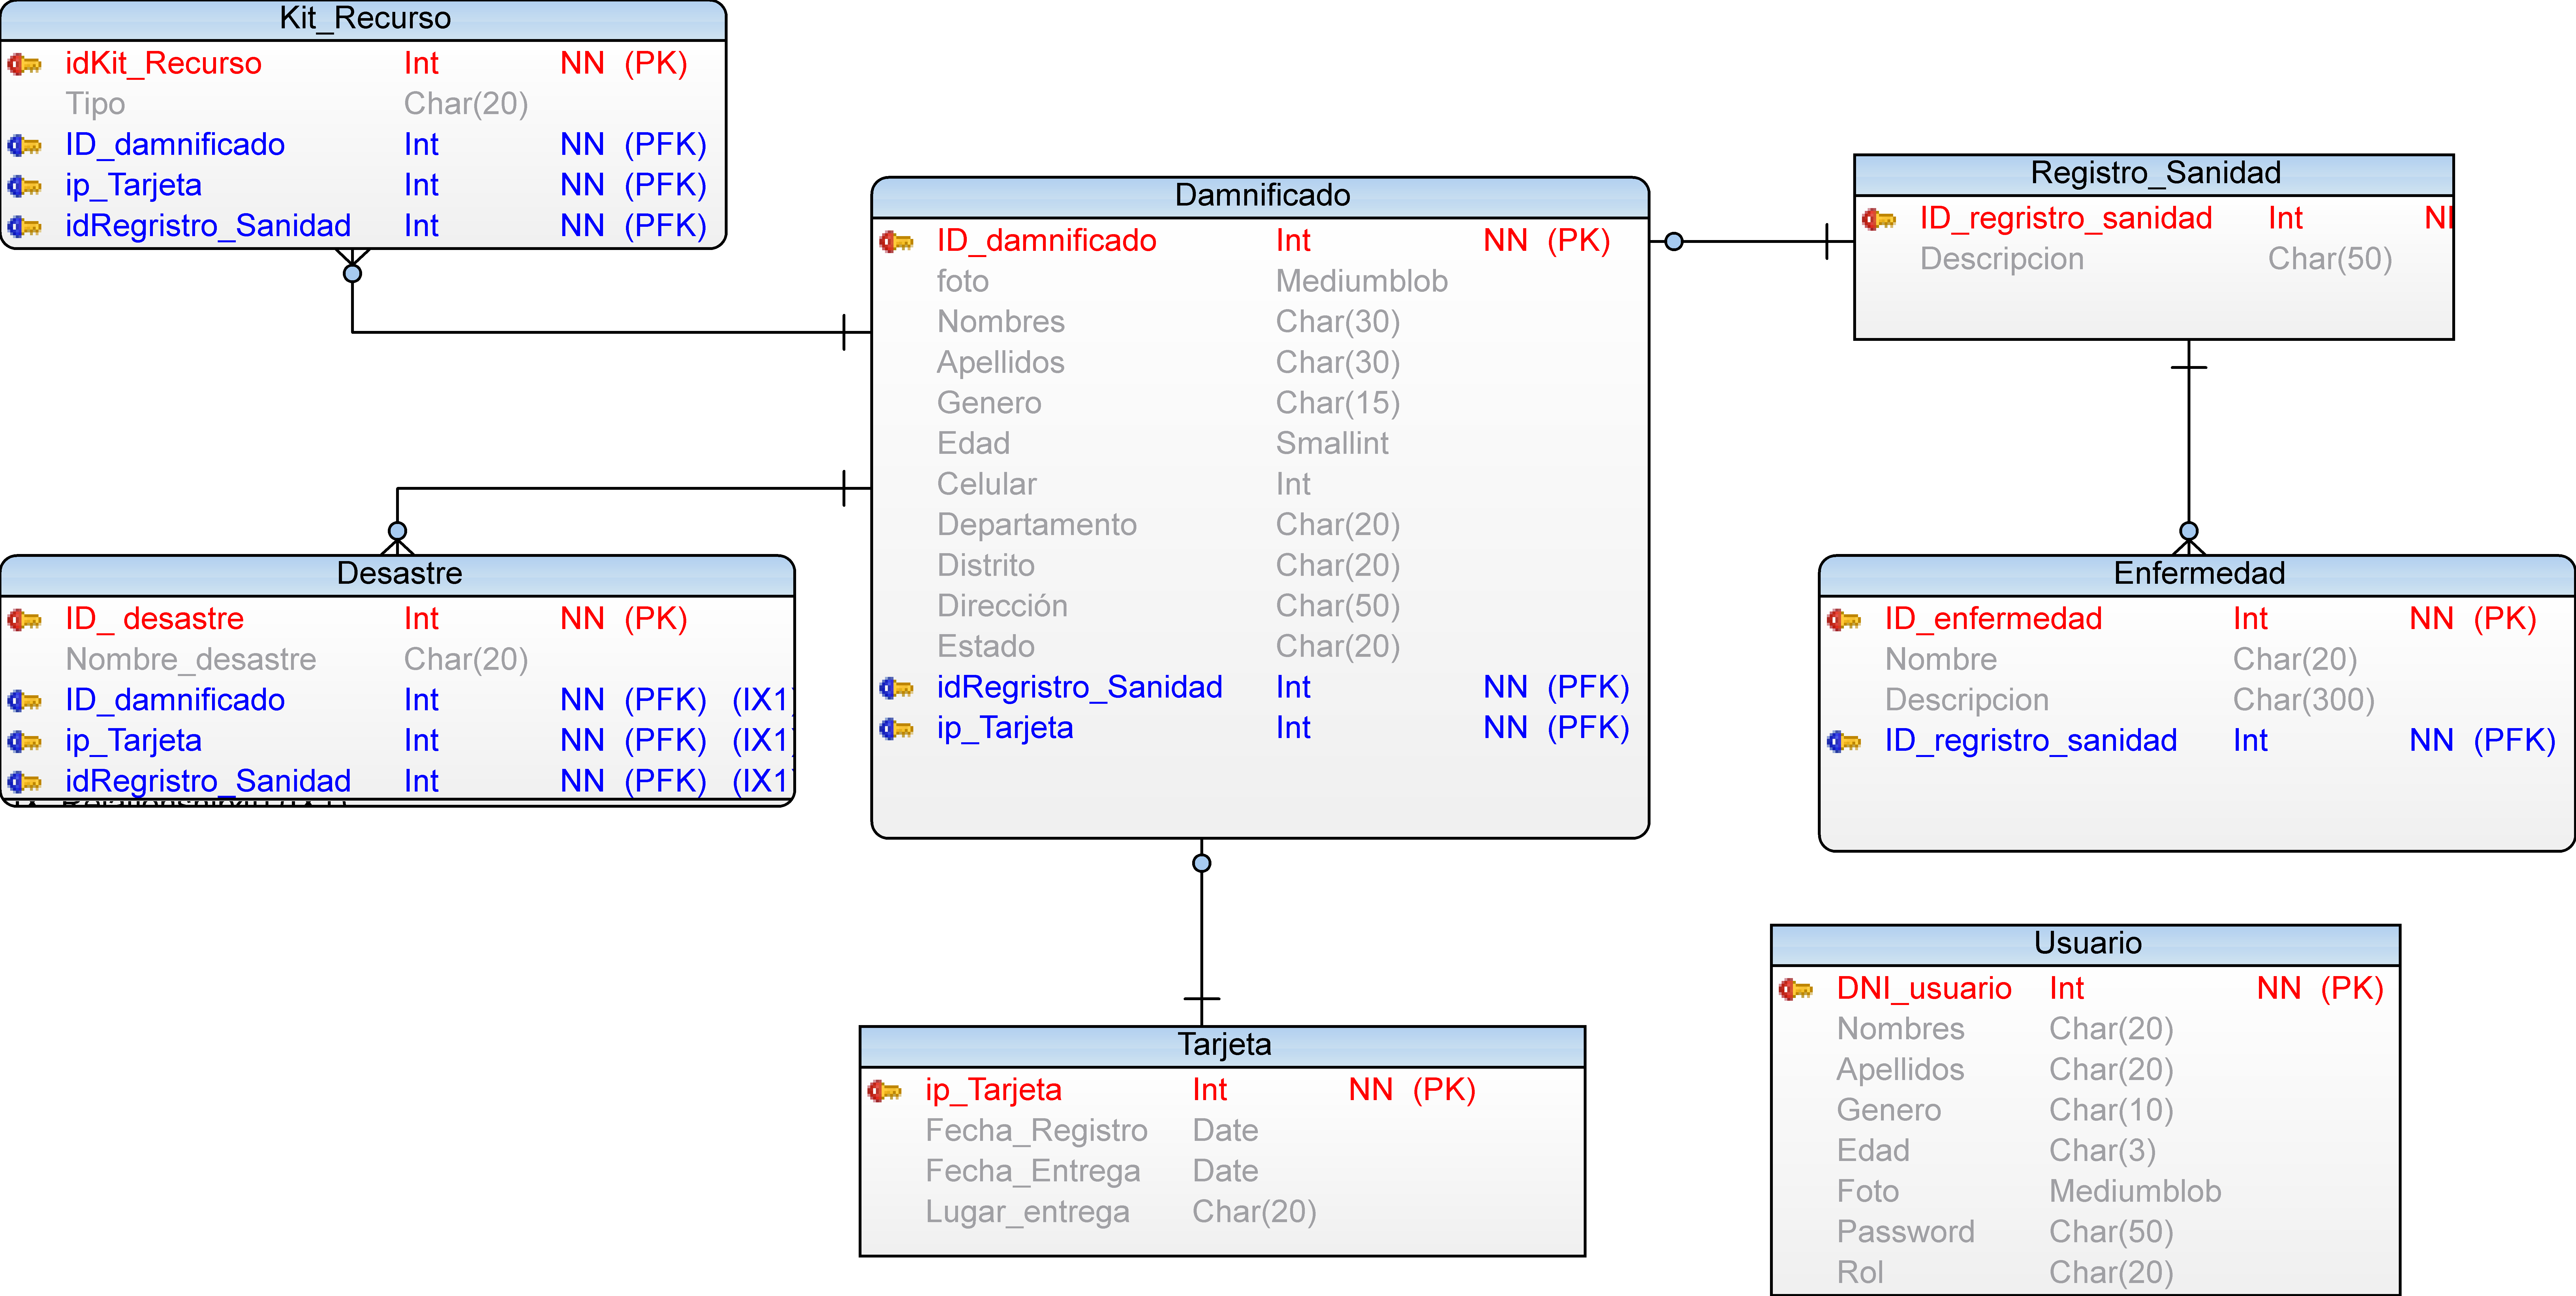
\includegraphics[width=1.1\textwidth]{imagenes/modelo_de_datos.png}
			\caption{Modelo de datos}
			\label{Modelo_de_datos}
	\end{figure}
	\newpage
	\section{Diagrama General}
	Se presenta un diagrama de como funcionaría el sistema explicado paso a paso.
	\begin{figure}[htbp]
			\centering
			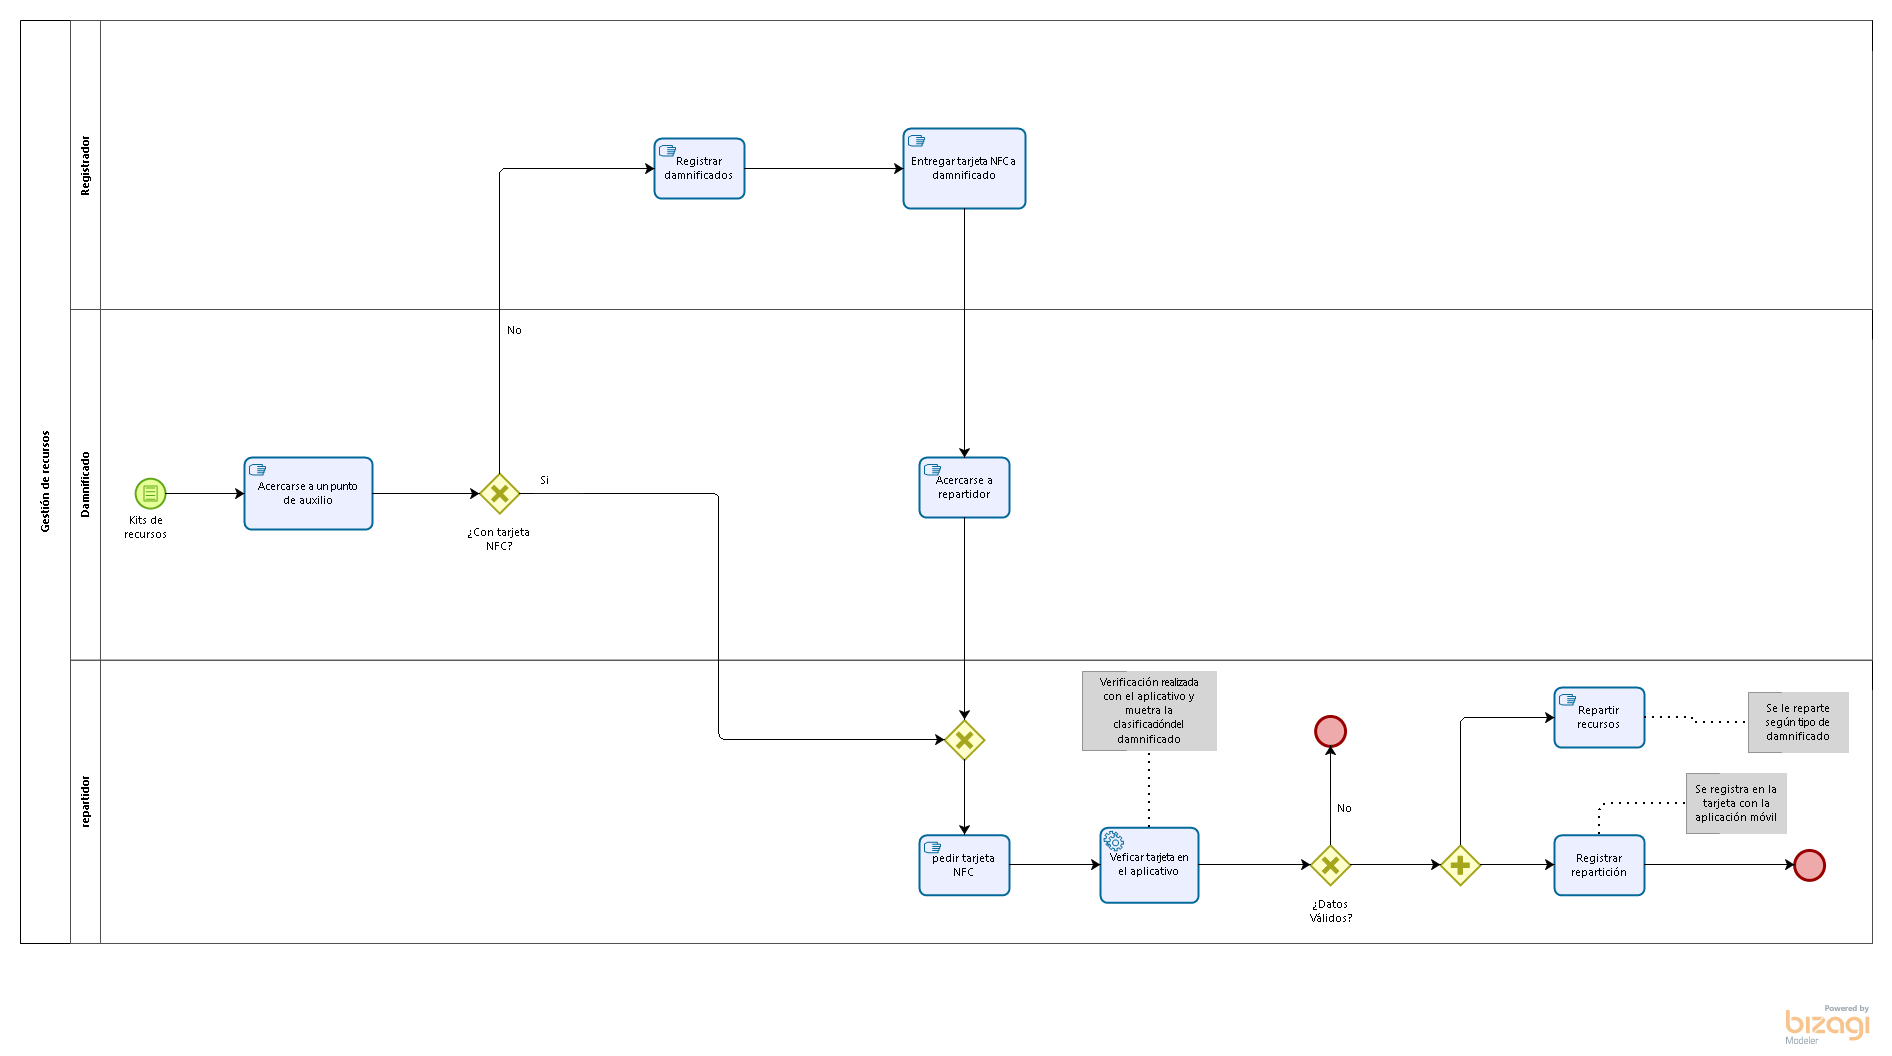
\includegraphics[width=1.2\textwidth]{imagenes/Diagrama_general.png}
			\caption{Diagrama general}
			\label{Diagrama_general}
	\end{figure}

	\section{Implementación}
	Para la implementación se seguirá la metodología ágil Scrum. A continuación se muestra el Backlog para el proyecto:
	\newpage
	\begin{figure}[htbp]
			\centering
			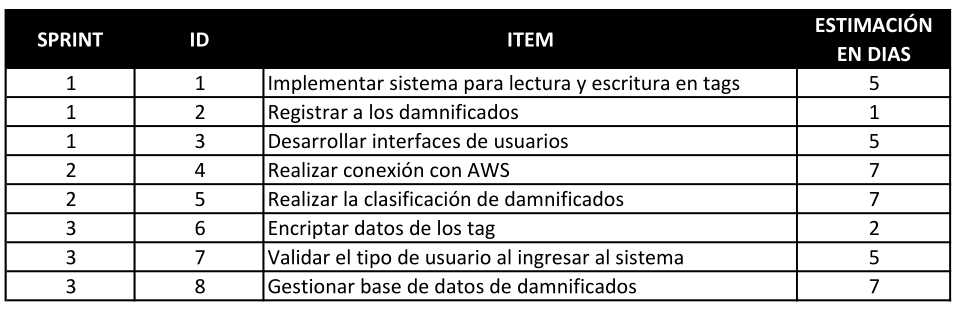
\includegraphics[width=1\textwidth]{imagenes/sprint.PNG}
			\caption{Product Backlog}
			\label{Product_Backlog}
	\end{figure}
	
	\bibliographystyle{ieeetr}
	\bibliography{biblio}
\end{document}